\documentclass[12pt,a4paper,openright,twoside]{book}
\usepackage[utf8]{inputenc}
\usepackage{disi-thesis}
\usepackage{code-lstlistings}
\usepackage{notes}
\usepackage{shortcuts}
\usepackage{acronym}
\usepackage{graphicx}
\usepackage{float}
\usepackage{subcaption}
\usepackage{enumitem}
\usepackage{cleveref}
\usepackage{url}

% Custom command for image source attribution
\newcommand{\source}[1]{%
    \vspace{-0.5em}
    \begin{center}
        \fcolorbox{white}{white}{%
            \parbox{0.95\linewidth}{%
                \small\centering\textit{Source:} #1
            }%
        }
    \end{center}
    \vspace{0.5em}
}

\school{\unibo}
\programme{Scuola di Ingegneria e Architettura \\ Corso di Laurea Magistrale in Digital Transformation Management}
\title{Observability through a telemetry framework for distributed web apps: error and performance monitoring for Technogym Mywellness CRM}
\author{Francesca Gaeta}
\date{\today}
\subject{BIG DATA AND CLOUD PLATFORMS}
\supervisor{Prof. Matteo Francia}
\cosupervisor{Dott. Davide Domini}
\session{II}
\academicyear{2025-2026}

% Definition of acronyms
\acrodef{CRM}{Customer Relationship Management}
\acrodef{OTel}{OpenTelemetry}
\acrodef{POC}{Proof of Concept}
\acrodef{PWA}{Progressive Web Apps}
\acrodef{KPI}{Key-Success Factors}
\acrodef{TBS}{Technogym Business System}
\acrodef{OTLP}{OpenTelemetry Protocol}
\acrodef{RUM}{Real User Monitoring}
\acrodef{UX}{User Experience}
\acrodef{APM}{Application Performance Monitoring}
\acrodef{OLTP}{Online Transaction Processing}
\acrodef{BI}{Business Intelligence}
\acrodef{OLAP}{Online Analytical Processing}
\acrodef{ACID}{Atomicity, Consistency, Isolation, Durability}
\acrodef{ETL}{Extract Transform, Load}
\acrodef{PaaS}{Platform-as-a-Service}
\acrodef{IaaS}{Infrastructure-as-a-Service}
\acrodef{FaaS}{Function-as-a-Service}
\acrodef{SaaS}{Software-as-a-Service}
\acrodef{XaaS}{Anything-as-a-Service}
\acrodef{VM}{Virtual Machine}
\acrodef{OS}{Operating System}
\acrodef{GDPR}{General Data Protection Regulation}
\acrodef{CWV}{Core Web vitals}
\acrodef{SLI}{Service Level Indicator}
\acrodef{SLO}{Service Level Objective}
\acrodef{RBAC}{Role-Based Access Control}
\acrodef{SRE}{Site Reliability Engineering}
\acrodef{MTTR}{Mean Time to Repair}
\acrodef{DOM}{Document Object Model}
\acrodef{CWV}{Core Web Vital}
\acrodef{API}{Application Programming Interfaces}
\acrodef{BE}{backend}
\acrodef{FE}{frontend}
\acrodef{CORS}{Cross-Origin Resource Sharing}
\acrodef{EoS}{End of Support}
\acrodef{GDPR}{General Data Protection Regulation}


\mainlinespacing{1.241} % line spacing in mainmatter, comment to default (1)
\setlength{\parskip}{1em}
\setlength{\headheight}{27.05003pt}

\begin{document}

\frontmatter\frontispiece

\begin{abstract}	
Modern distributed systems and microservices architectures present unprecedented challenges for enterprises in understanding application behavior in production. Traditional monitoring approaches, that rely on known failure modes, are insufficient to face the unpredictability of contemporary digital ecosystems. Imagine monitoring an e-commerce to recognize when the API dedicated to payments is being slower than usual. Basic monitoring can intercept the existence of the issue, but not rebuilding the reasons behind it, which has to be investigated manually. This is the reason why observability has emerged to support digitalized companies in this situation, since it is capable of inferring internal system states from external outputs such as logs, metrics and traces, without any prior knowledge of specific failure scenarios. In this context, considering the same anomaly for the e-commerce, the system allows noticing that the slowdown only involves European users, or that after the latest deployment something changes in the indexes used for the query and this brought a worsening of the service. Developers can save time and effort if guided by this bunch of data that walk the path back. 
This thesis explores the practical implementation of observability frameworks in enterprise contexts, addressing the fundamental shift from reactive troubleshooting to proactive system intelligence evaluating modern observability platforms. Technogym Spa serves as case study for this research. Specifically, the core in terms of customer care was providing users with high quality digital products and assistance. Before this infrastructure, the customer experiencing a problem while using the CRM services had to report it to the technical assistance. Even though developers were fast in solving the errors respecting the one-day deadline - especially for the ones classified as high criticality -, the whole process to make them aware of the alert expanded the time window during which the client could not access the broken parts of the application, lasting even days. They wanted to avoid it to add more value to the customer.
The implementation focuses on the Mywellness CRM Progressive Web Application, demonstrating how observability principles can be applied to React-based frontend applications to enable proactive error detection and performance optimization while respecting strict privacy regulations.
\end{abstract}

\begin{dedication} % this is optional
Cadendo, la goccia scava la pietra, \\ non per la sua forza, ma per la sua costanza.
\end{dedication}

%----------------------------------------------------------------------------------------
\tableofcontents   
\listoffigures     % (optional) comment if empty
\lstlistoflistings % (optional) comment if empty
%----------------------------------------------------------------------------------------

\mainmatter

%----------------------------------------------------------------------------------------
\chapter{Introduction}
\label{chap:introduction}
%----------------------------------------------------------------------------------------

The landscape of enterprises, especially the highly technological ones, or those strictly related to software development, has undergone a radical transformation over the past two decades. Organizations have progressively migrated from monolithic applications where all functionalities resided within a single codebase, toward distributed architectures composed of numerous microservices dedicated to different business capabilities. This evolution was driven by the need for independent scalability of different application components, the ability to deploy updates without system downtimes, the flexibility to adopt diverse technology stacks optimized for specific tasks, and the organizational agility to enable autonomous teams working on different services simultaneously. \\ Furthermore, the adoption of cloud computing platforms intervened in decoupling infrastructures to overcome strict hardware constraints and pushing towards horizontal scaling and global distribution. This elasticity introduced a new dimension of operational complexity driven by a multiplied number of components, their interactions, and potential failure points. 

All things considered, traditional monitoring paradigms were designed for a simpler era. These systems operate on the principle of \textit{known unknowns}, which means they excel at answering specific, predefined questions, and monitoring tools rely on static dashboards configured based on historical failure modes that engineers have previously encountered and explicitly instrumented. However, we can spot emergent behaviors that cannot be predicted by examining individual components in isolation. Failure modes became unpredictable and cannot always be anticipated by simple static alerts, entering the era of (\textit{unknown unknowns}). For instance, a performance degradation might be due to the interplay of multiple factors, such as network latency and database query optimization, therefore it comes to help to dispose of a kind of information that lets us walk the path back to explore the plausible chain of problems. Traditional monitoring falls short in this scenario because no one would have thought of those possibilities that generated the error. \\ The business impact of this monitoring gap is substantial. Apart from causing higher costs for the company, slow page loads, unresponsive interfaces, intermittent errors, erode user trust gradually, and we only discover it not thanks to metrics, but when we observe the abandonment rate increasing. For organizations competing in digital markets, the ability to rapidly diagnose and resolve issues directly translates into competitive advantage. 

For a global leader such as Technogym, where the intersection of high-end industrial manufacturing and sophisticated digital ecosystems creates a unique, wide operational environment, this shift is determinant. Through observability, rather than trying to predict any possible scenario - which is basically impossible -, we can focus on ensuring the systems emit rich telemetry data to recognize anomalies a posteriori. The true power of this technique emerges from the correlation of three essential signals that we will better disclose throughout the thesis: metrics, logs and distributed traces. In the examined case study, we will document the implementation of a project aimed at enhancing error monitoring and system performance declined for the corporate Mywellness CRM app. By leveraging the \ac{OTel} framework, alongside AI-driven correlation analysis, we can transform raw telemetry into actionable insights. This shift from reactive troubleshooting to predictive maintenance represents a significant value-add for the Technogym's ecosystem, ensuring that \textit{Wellness} remains a seamless experience across both physical and digital domains.  

\par The research is organized as follows:
\begin{itemize}[nosep]
    \item \textbf{Chapter 2:} provides an overview of Technogym’s corporate philosophy and internal digital processes, highlighting the cultural drive for constant innovation. We will get acquainted with the project. 
    \item \textbf{Chapter 3:} explores the theoretical foundations of \textit{observability}, focusing on the \ac{OTel} standard and a comparative analysis of modern monitoring platforms to identify the most suitable solution for the enterprise context. 
    \item \textbf{Chapter 4:} details the practical implementation of the infrastructure from the initial \ac{POC}, an experiment conducted to validate the feasibility, functionality, and potential of a technology, to the integration of custom libraries. We will dive into the code architecture to understand how monitoring is enabled and integrated in the app. 
    \item \textbf{Chapter 5:} analyzes the project's primary outcome, a robust error-monitoring system. It discusses the technical hurdles, \ac{KPI} definition, and the resulting improvements in incident response.  
    \item \textbf{Chapter 6:} ((to decide)). discusses secondary project outputs, including performance benchmarking, user behavior analysis via heatmaps, and long-term usage statistics (IF I HAVE TIME AND ROOM and depends on when the project is complete). 
    \item \textbf{Chapter 7:} concludes the thesis with a reflection on the potential future evolution of the project and the professional and personal growth achieved during the internship.
\end{itemize}

\chapter{Technogym: the wellness ecosystem}

In Technogym, innovation is not a destination, yet a constant state of motion. A recurring sentiment within the company is that ``once a goal is reached, it is already part of the past''. This is the motivation that makes it outperform competitors and positions it as one of the most influential wellness companies in the market, as recently stated by the \textit{TIME Magazine}. 

Founded in 1983 by President Nerio Alessandri and headquartered in the Technogym Village in Cesena, the company has consistently redefined the boundaries of the ``Wellness'' experience. However, in an era where digital touchpoints are as critical as physical equipment, the company’s ambition has shifted to ``proactive'' excellence. The goal is no longer just to provide a high-quality interface, but to achieve a level of operational transparency where bugs or performance regressions are intercepted before the user even perceives them. Ideally, issues should be identified and resolved before a customer even feels the urge to contact support. 
\\ The company’s DNA is built on the concept of the \textit{Wellness Valley}, which integrates physical health, mental well-being, and technological innovation. Internally, this translates into a high-precision work environment where automation and digital documentation are paramount.

There are four main words to identify Technogym's drivers: 
\begin{enumerate}[nosep]
    \item \textbf{Technology}, which seems quite trivial considering the world that Technogym has created and the reality we live in right now, but in 1989 it was totally visionary. Technogym always led technology-driven changes in the fitness industry, setting high standards for equipment built by other companies. Nowadays, enterprises are considering digital transformation and are always more prepared to face innovation, which might put Technogym in a bad spot, and this is the reason why it always thrives with newer solutions and endless enhancement to protect its relevance and leadership. 
    \item \textbf{Personalization}, what motivates the users to start a training program with the aid of the app through which they can get in touch with professionals based on their requests, routines and, most importantly, unique needs, assigning customized programs for a highly personal experience.
    \item \textbf{Health}, which is the most emphasized part of the life of people. Technogym pushes it at the vertex of the pyramid, without forgetting other important aspects such as amusement, passion, socialization, strength, and aesthetic purposes. 
    \item \textbf{Ecosystem}, probably the real essence that encloses it all. Technogym was the first to introduce a \textit{digital key} to access its machines with a user account where all personal data and training progress are collected, to then switch to the modern web applications released either for professional operators in clubs, hotels and hospitals who need to follow their clients, and for common people that want to gain access to a training program in an easy and efficient way to improve their lifestyle and habits while feeling assisted; it was the first to make clever usage of the cloud when it was first developed to really become seamless.
\end{enumerate}

\section{A React-based implementation framework for observability: the project for the \\ Mywellness CRM web application}

Technogym operates as a hybrid of a hardware manufacturer and a software house, thus are we interested in grasping the context around the Mywellness CRM, the application the project was tailored on, to understand its functioning and the weak points the development team wanted to intervene on in order to boost customer experience and accelerate the debugging process. 

The Mw-CRM is a \ac{PWA} that enables fitness professionals to manage client relationships, design personalized training programs, track progress, and deliver engagement through web and mobile interfaces. \cite{webdev-pwa} \ac{PWA} are web applications built and enhanced with modern APIs to provide enhanced capabilities while still reaching any web user on any device with a single codebase. Reliable apps also need to be usable regardless of network connection. Users expect apps to load quickly on slow or flaky network connections, or even when offline. Making the PWA installable moves it out of the browser and into a standalone window. Installed PWAs can be launched on the user's home screen, dock, taskbar, or shelf. The user can search for them on a device and jump between them with the app switcher, making them feel like part of the device they are installed on.

The CRM platform is designed to be used by professionals who support their clients during their training journeys. It should not be confused with the well-known Technogym App, which is instead the mainstream app for very final users who train in the gyms around the world, yet the CRM is the bridge such facilities and their operators have to reach and guide their clients during their workouts and fitness journeys, even by exploiting the Technogym App itself (for instance, messages and updates can be sent directly there). With seamless integration of third-party software, smart equipment, and wearables, Mywellness (\cref{crm}) puts operators in full control of their digital strategy and members engagement. It is statistically measured to increase attraction of 40\% and retention of 30\% thanks to variety, customization and automation. More than 30 thousand facilities and 40 million users are registered on the platform, with more than 500 thousand workouts tracked. The application is extremely complex due to its level of detail in covering a huge number of cases and functionalities. The workflow it follows consists of an ensemble of subsequent steps, starting from collecting health and fitness information to build the user's health history, then offering direct booking of courses/trainers and payment possibilities, defining the assessment to discover the user's goals and consequently building the best personalized training program, consistently tracking progress, offering communication channels through which coaches can stay in touch to motivate clients, creating challenges to encourage friendly competition and keep users engaged, and finally rewarding results and loyalty. The Mw-CRM requires frontend programming expertise, but something fascinating about the observability project itself was that it could be interpreted as a ``backend solution for the frontend'', involving a combination of both, even without directly intervening on BE components as APIs or databases. 


\begin{figure}[H]
    \centering
    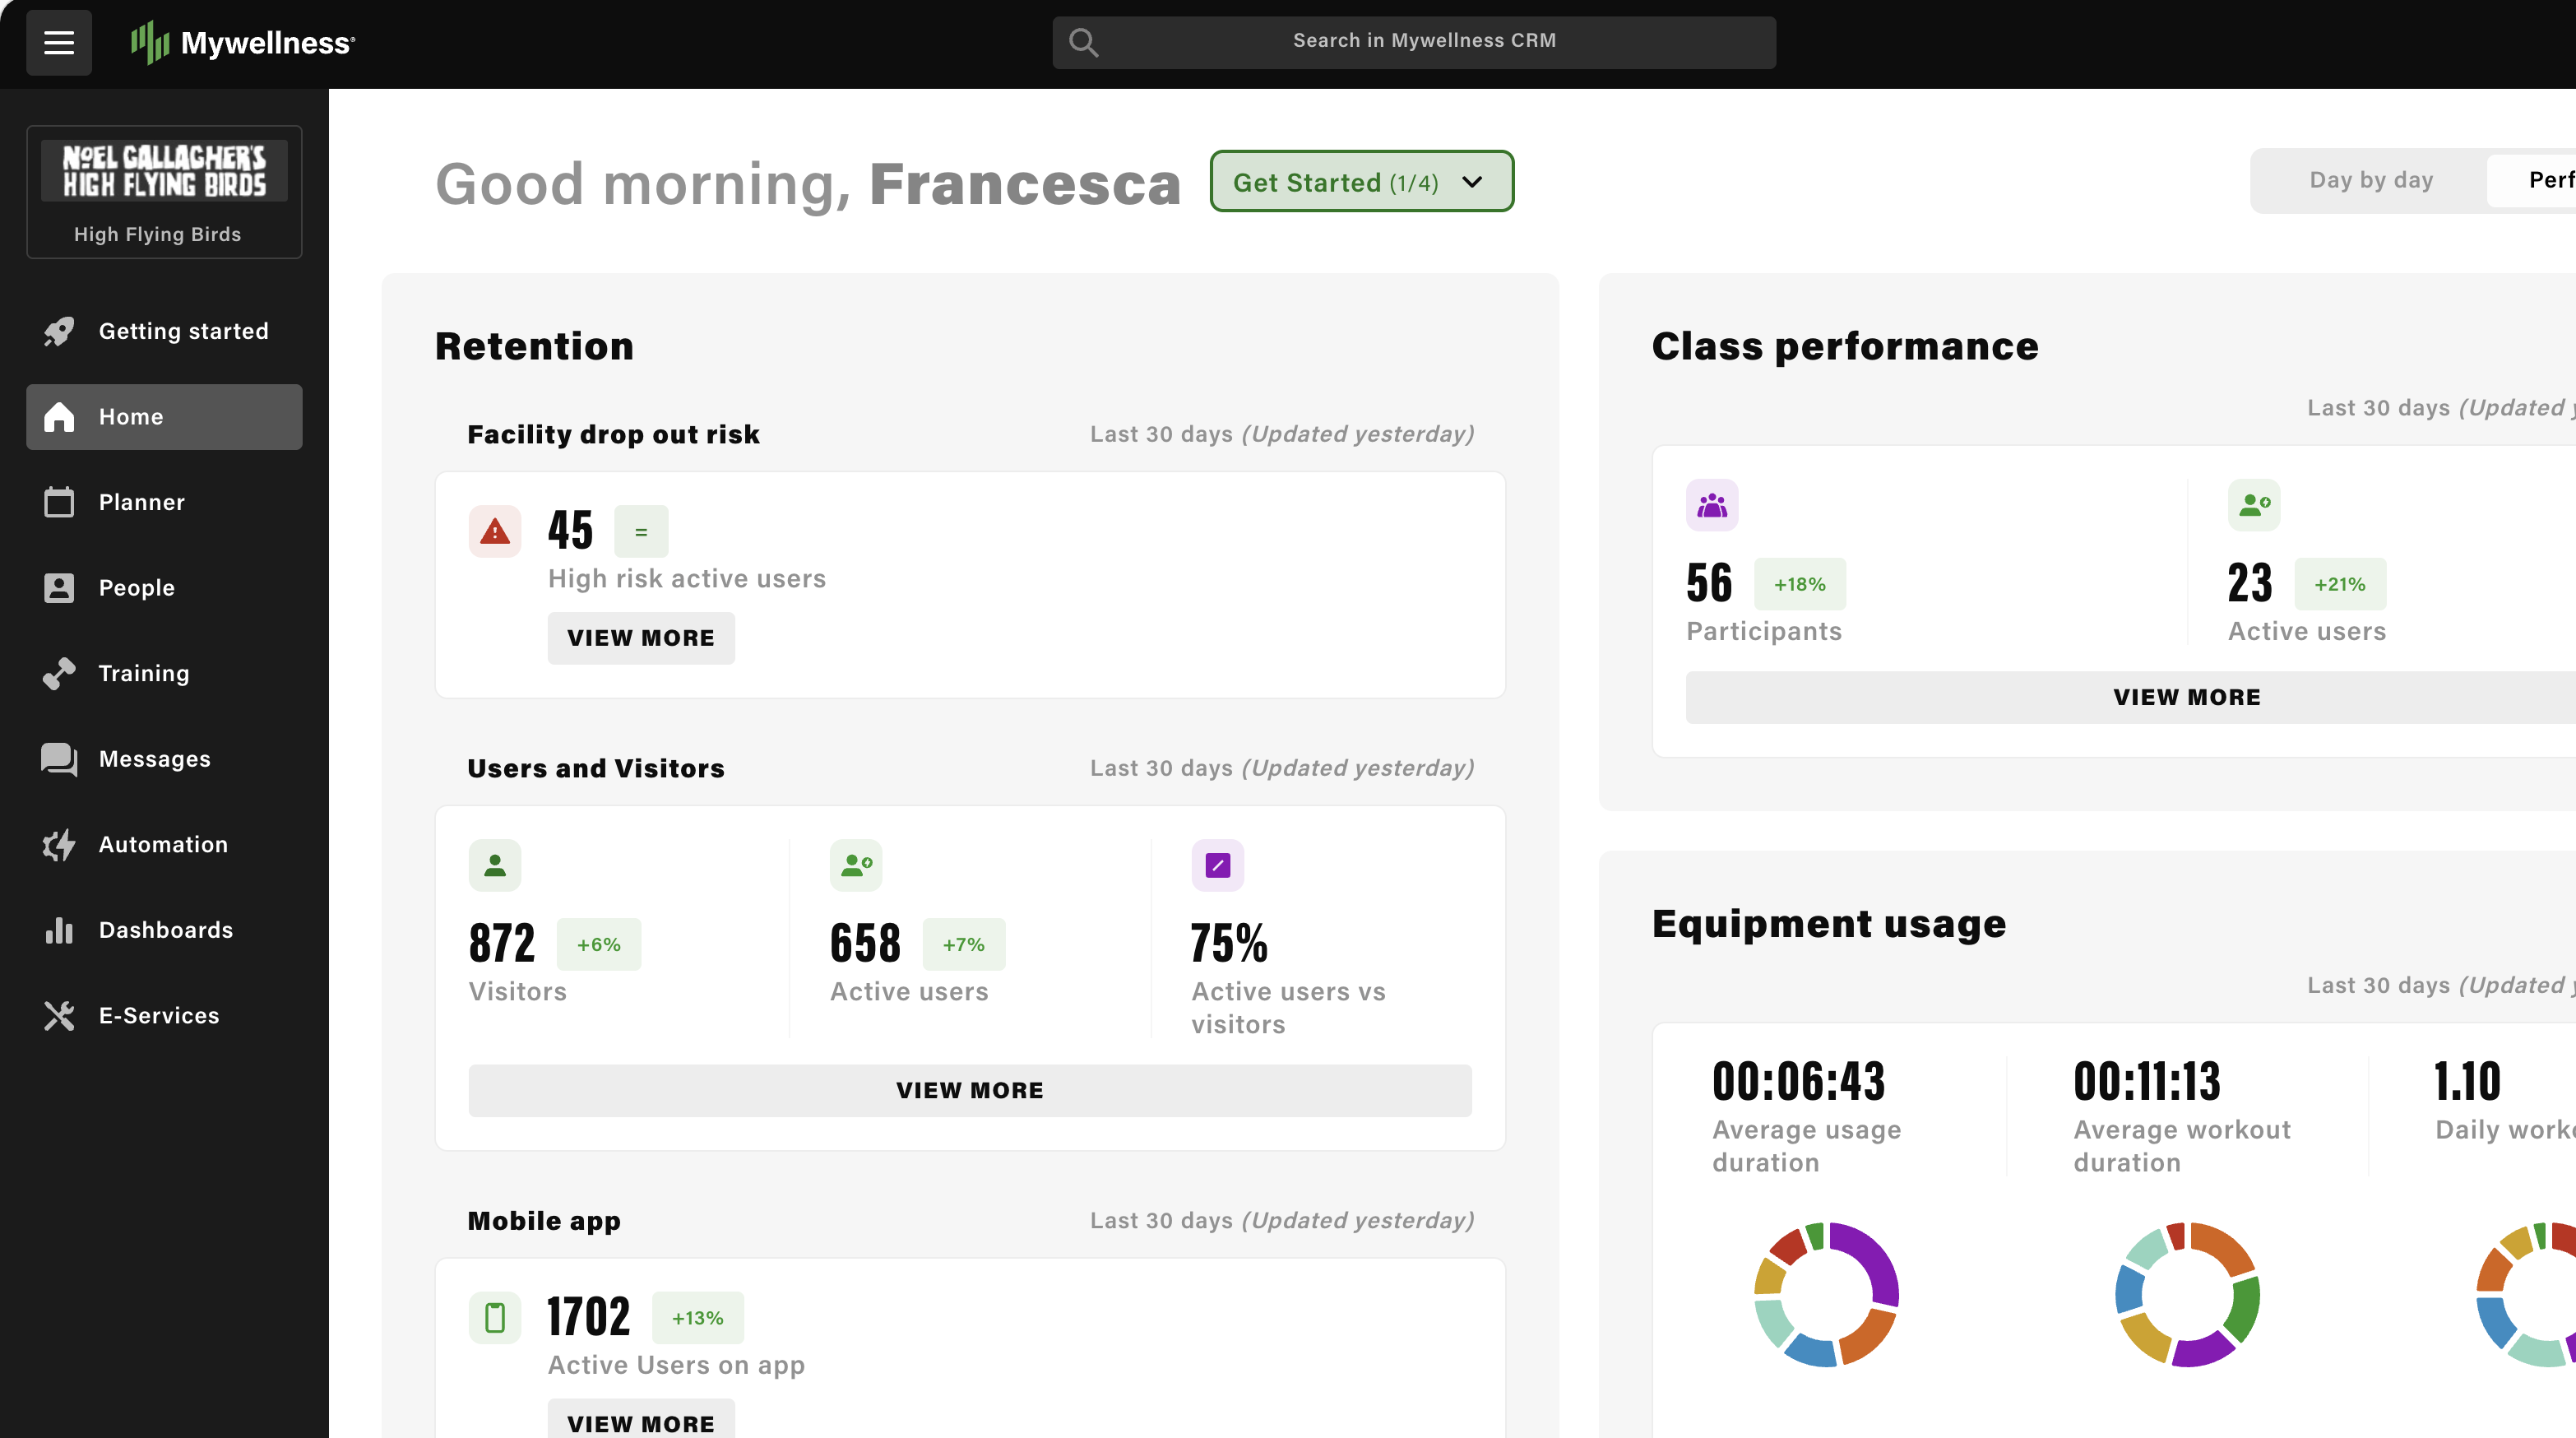
\includegraphics[width=1\linewidth]{figures/crm app.png}
    \caption{CRM Web App: Home Page}
    \label{crm}
\end{figure}

All the services, platforms and processes mentioned in broad terms in these sections underline the transition trend from traditional manufacturing to a digital-first approach that already began years ago. The frontend team continuously works to redesign the interface when it can be elevated, listens to and satisfies customers' requests and suggestions that would make their sessions in the gym better, and of course it must solve bugs and errors. It is fundamental to put the accent on these tasks to concretize the ``The Present is Already the Past'' mindset, possibly linked to the need for observability: to stay ahead of the market, the infrastructure must be self-aware and constantly evolving. One of the best ways to do so is to introduce tools and tune AI systems to automate and speed up workflows and problem resolution, while acquiring insights about what has changed with respect to previous versions, or years, or functionalities. The right data to nourish this whole workflow can be collected by exploiting observability principles, that we are going to officially disclose in the next chapter as focal point of the paper. 

In relation to what we illustrated until now, the request Technogym advanced was to create a complete and reusable library for \textbf{React} and \textbf{TypeScript} applications that enables application observability management through a single integrated platform. The library must collect and transmit telemetry data using the OpenTelemetry protocol to monitor errors, performance, user interactions, and usage statistics. The reason for implementing a library is that, ideally, observability could be considered exclusively a CRM goal at first, to then be expanded to other digital products just by importing it. 

As main features, we find:
\begin{itemize}[nosep]
    \item \textbf{Error Monitoring:} automatic capture of JavaScript errors, React error boundaries, API calls, complete stack trace tracking, handling of asynchronous errors and promise rejections, error categorization and prioritization. This initial phase covers the internship period and the main deliverables the company committed to guide me through.
    \item \textbf{Performance Monitoring:} Core Web Vitals measurement (LCP, FID, CLS), page and resource loading time tracking, React component rendering performance monitoring, API call response time analysis, threshold definition for sending alerts via email or Slack messages;
    \item \textbf{Heatmaps and Scrollmaps:} recording of user click positions, heatmap generation to visualize most interacted areas, page scroll depth tracking, navigation and interaction pattern analysis;
    \item \textbf{Usage Statistics:} collection of browser information, version, and user agent, user geolocation (country, region), device data (desktop, mobile, tablet) and screen resolution, engagement metrics (time on page, bounce rate), tracking of visited pages and navigation paths, event tracking to evaluate feature usage.
\end{itemize}

The technology stack is expected to include version 18+ of React and 5+ of TypeScript for the frontend, OTLP as telemetry protocol, Vite as build tool for library bundle creation, Vitest for testing and Vite Plus with OXLint for linting and formatting, which concerns the process of running a program that will analyze code for potential errors. Linting focuses on enforcing coding conventions and best practices, detecting syntax errors and improving code readability as a sort of static analysis to catch issues early to maintain code consistency and clarity. Testing, whose debugging is a synonym, involves manually fixing the code after a bug has been found, generally after the program has run, and this differentiates it from the linting practice. This latter, before was implemented through the \textit{ESLint} library for the validation part, and the \textit{prettier} library for the formatting part, and thanks to plug-ins they could function simultaneously. Now, they switched to \textit{Vite Plus} with \textit{OXLint} because claimed to be up to 40 times faster and more powerful than traditional systems. Integrating a single package instead of keeping both ESLint and Prettier will reduce configuration conflicts and dependency vulnerabilities. 

The workflow is intended as follows:
\begin{itemize}[nosep]
    \item \textbf{Phase 1.} In depth analysis of OpenTelemetry and its APIs, study of existing libraries and backend platforms to define the architectures to implement.
    \item \textbf{Phase 2.} Core implementation (with precedence to error tracking) to achieve the goals and observe the requirements mentioned above, adding the development of precise unit tests to simulate errors to check if they are collected in the platform. The idea is to start from a blank template that will be modified according to our needs to test if what we are building works before migrating everything to the real application. 
    \item \textbf{Phase 3.} Configuration of dashboards to monitor errors in the platform, and of alerting systems to notify errors from the platform.
    \item \textbf{Phase 4.} Structuring the README file, API documentation and minimal demo app. 
    \item \textbf{Expected Deliverables.} A library source code published on Git repository, npm package ready for distribution, a complete technical documentation, a working demo application, a test suite with at least 80\% coverage and a presentation to show results. 
\end{itemize}

Each step will be further analyzed and understood as the reading proceeds in the designated parts. 

\chapter{From simple monitoring to observability in distributed systems}

\cite{observability} Historically, system health was managed through \textit{monitoring}, a reactive process centered around ``known unknowns''. Monitoring tools are designed to answer specific questions, like discovering if the server is up, or the CPU usage percentage. These rely on predefined dashboards built upon failure modes that engineers have encountered before, which also means that we cannot monitor something we do not know the existence of, or something we have not set as threshold. Modern software architectures require more than just monitoring; they require \textit{observability}, the ability to understand a system's internal state solely from its external outputs (logs, metrics, and traces). Technogym needed this as it transitioned into a distributed system of microservices and cloud-integrated fitness equipment, and failure modes became unpredictable and cannot be anticipated by simple static alerts (\textit{unknown unknowns}). 

In an observable system, we do not just wait for a threshold to be crossed; we collect enough granular data to understand why something is happening for issues we have never experienced before. For the Mywellness CRM app, this means the difference between knowing the app is slow and knowing that a specific API call is lagging for users on a specific firmware version in a specific region. Capturing various severity level types for logs (e.g., error, info, warn, ...); associating types of data with personalized message bodies to understand in natural language what crashed; building dashboards and reports; these all embody strategies to speed up the correction of bugs and malfunctions. 

To achieve this level of insight, the industry relies on three fundamental types of telemetry data that we wanted indeed to intercept for the project \cite{observability}:
\begin{itemize}
    \item \textbf{Metrics.} Metrics are numerical representations of data measured over intervals of time. They are incredibly efficient for storage and ideal for spotting trends or triggering alerts. In the Technogym ecosystem, metrics might track the number of active workouts per second or the memory consumption of a \ac{CRM} background process. They cause low overhead and retention is set to the long-term, but they are not enough alone to understand the context, since they just warn when \textit{something} is wrong, but not \textit{where} or \textit{why}.
    \item \textbf{Logs.} Logs are timestamped text records of discrete events. They provide the report of a failure. Whether it is a 404 error on a login page or a database connection timeout, logs offer the specific details needed for debugging. They are pricier to store and difficult to search at scale without proper indexing. It is not compulsorily associated to a predefined user, this is the reason why it should be correlated to other measurements.  
    \item \textbf{Traces.} Distributed Tracing is arguably the most critical pillar for modern apps like Mywellness. A trace follows a single request as it travels through various services (e.g., from the user's smartphone to the authentication layer, then to the database, and back). It provides a map of the journey, highlighting exactly where delays or errors occur. Traces show the exact path and timing of service calls, reveal dependencies between services, highlight performance bottlenecks, and provide context about each step in a request's life cycle, this is why traces and logs become extremely powerful if coupled up. 
\end{itemize}

There are other kinds of information we can acquire thanks to \textbf{spans}, that are single units of work and track specific operations that a request makes (actually a trace can be composed of one or more spans), and there is a whole table of attributes available to cluster spans, or \textbf{events} as structured records of significant occurrences in the system, or \textbf{profiles} that provide deep analysis of resource consumption and code execution patterns, but the ones in the paragraph above are the most important ones which automatically link to these various subcategories.  

\section{The role of OpenTelemetry}

OpenTelemetry has emerged as the industry's answer by offering a unified framework for collecting and managing observability data. It focuses on the collection, processing, and export of telemetry data, leaving the monitoring and alerting aspects to other observability tools. Its strength is being an open-source and vendor-neutral framework that standardizes how we collect and handle telemetry data across distributed systems \cite{OpenTelemetry}. 

The vendor neutrality approach extinguishes a major problem in modern observability: the fragmentation of telemetry collection methods. Instead of maintaining a different instrumentation code for each monitoring tool, we can instrument with \ac{OTel} the first time and send data anywhere, instead of managing different pipelines for logs, metrics, and traces. It acts like a common language for observability data that works across all services, regardless of the programming language. We must be aware that this library is not a monitoring or alerting tool itself, yet it provides the means to collect telemetry data from applications without built-in monitoring capabilities that we should tune externally. 

Other important aspects are the preservation of backward compatibility with existing implementations. Before, vendor dependency led to using fragmented tools with different languages and proprietary agents and high maintenance overhead, but with OpenTelemetry everything is unified and language-agnostic. \ac{OTel} uses the \ac{OTLP} to move data between components. \cite{OTelCollector} The hint from the previous considerations is that the library does not immediately offer a storage, but we can agglomerate to our architecture any type of instrument, like the \textit{OTel Collector} in a natural way that acts as a central hub. It takes in telemetry from different sources (not just OpenTelemetry SDKs, but also Zipkin, Prometheus etc.), processes it, and sends it wherever, which means we do not need to hard-wire the application to any backend. The collector is in charge of routing, formatting and cleaning up, and it can run in different modes: in \textit{agent mode} it runs on the same machine as the app and filters or enriches data before sending it out; in \textit{gateway mode} it runs as a central service that collects telemetry from multiple apps or instances. Nothing prohibits to use both, therefore collect locally and then forward centrally. 

The collector (\textit{\cref{collector}}) works as a modular pipeline with four key components: 
\begin{itemize}[nosep]
    \item Receivers that handle incoming data from various protocols
    \item Processors that modify, filter, or batch data
    \item Exporters that send processed data to different backends
    \item Connectors that pass data between pipelines or generate new telemetry types 
\end{itemize}

\begin{figure}[H]
    \centering
    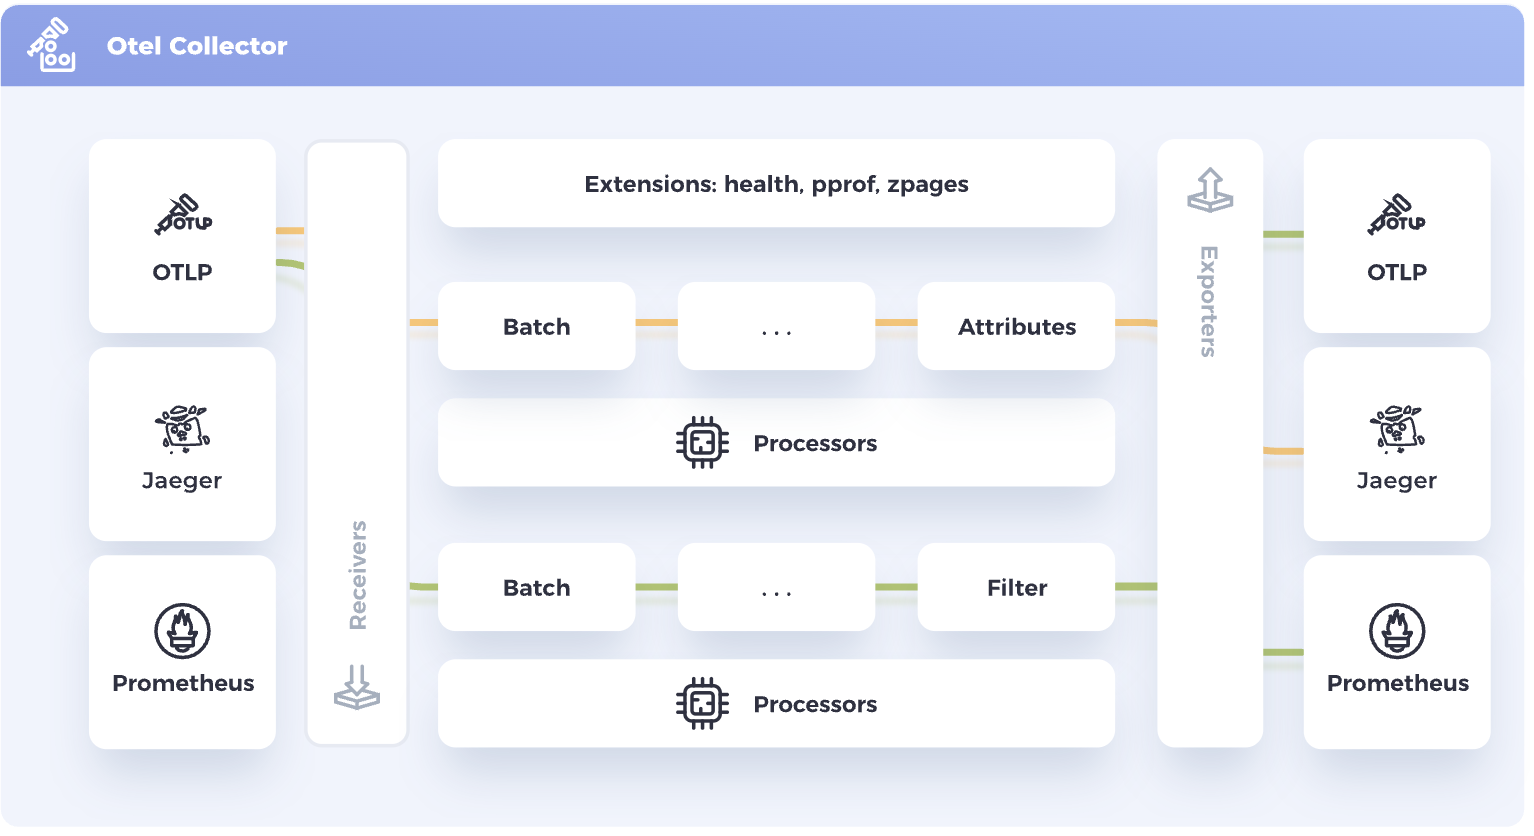
\includegraphics[width=0.9\linewidth]{figures/collector.png}
    \caption{OpenTelemetry Collector Architecture.}
    \source{https://opentelemetry.io/docs/collector}
    \label{collector}
\end{figure}

For getting started with OpenTelemetry, sending data directly to a backend is a great way to get value quickly. Also, in a development or small-scale environment - which is not our case -, we can get decent results without a collector. However, it is recommend using a collector, since it allows the service to offload data quickly and the collector can take care of additional handling like retries, batching, encryption or even sensitive data filtering. Since standardization of movements does not tie to any vendor, if we need to switch tool we just update the collector's configuration in one line.  

\section{Possible limitations in OTel}

While OpenTelemetry provides a robust framework for digital transformation, its implementation is not exempt from significant trade-offs. For a complex ecosystem like Technogym's, several inherent limitations must be addressed \cite{OTelLimits}. 

The act of observing a system inevitably consumes resources. Instrumenting applications with OTel SDKs introduces CPU and memory overhead, as the application must now generate, buffer, and export telemetry data. In high-throughput environments, such as processing thousands of simultaneous workout heart-rate samples, the ``observability tax'' can impact the very latency we aim to measure. This requires careful tuning of sampling rates to balance data depth with system performance. 

Observability shifts the burden from ``not having enough data'' to ``having too much''. Traces and logs, especially when highly granular, generate massive volumes of data. Storing and indexing this information in backends can lead to skyrocketing infrastructure costs. Without a clear sampling strategy where only a percentage of successful traces are kept while 100\% of errors are captured, the project risks becoming financially unsustainable.

Simply collecting the three pillars is insufficient; the true value lies in their \textbf{correlation}. If a log entry cannot be linked to a specific trace ID, or a metric spike cannot be drilled down into a trace, the data remains siloed. Ensuring that all microservices correctly propagate context across different programming languages and protocols is a significant engineering challenge that requires strict organizational standards.

It is critical to reiterate that OpenTelemetry is a collection standard, not a storage or analysis solution. While OTel unifies how data is sent, it does not provide the \textit{single pane of glass} for viewing it. Technogym must still maintain and manage backend databases and visualization layers. Furthermore, as \ac{OTel} is a relatively young and rapidly evolving project, certain components (specifically the logging specification and profiling) are less mature than tracing and metrics, potentially leading to breaking changes during future updates.

Finally, the transition to observability is as much a cultural shift as a technical one. Engineers must move away from ``dashboard-watching'' toward ``exploratory debugging''. This requires a deeper understanding of the system architecture and a new set of skills in querying high-cardinality data, which may initially slow the development speed during the adoption phase. 

\section{Platform Architectures: evolution from On-Premise to Cloud}

\ac{OTel} is excellent for standardized telemetry collection. However, the requirements in our project include \ac{RUM} and \ac{UX} analytics features that are not universally covered by OTel-compatible vendors, especially heatmaps and scrollmaps. In practice, most teams end up choosing:
\begin{enumerate}
    \item an observability backend that supports \ac{OTel} well, and
    \item optionally a UX/session analytics tool for dashboards and heatmaps, due to the fact that many \ac{APM} vendors do not do it specifically. 
\end{enumerate}

Today, OTel can correctly cover errors, performance and cross-signal correlation, but it does not natively provide heatmaps and scrollmaps, visual \ac{DOM} snapshots, product analytics funnels, retention and cohorts. We can add it thanks to other vendors. Hence, it is essential to identify the critical aspects and distinctions among typologies of platforms to effectively assess the solutions currently available on the market.

The point of interest is that, from the very beginning, data management was centered around the \textit{Relational Data Model}. These systems are designed for Schema-on-Write, meaning the data structure must be strictly defined before any information is ingested. Also, primordial databases were optimized for \ac{OLTP}, therefore daily operational tasks (e.g., updating a user's weight in a \ac{CRM}). 
\begin{figure}[H]
    \centering
    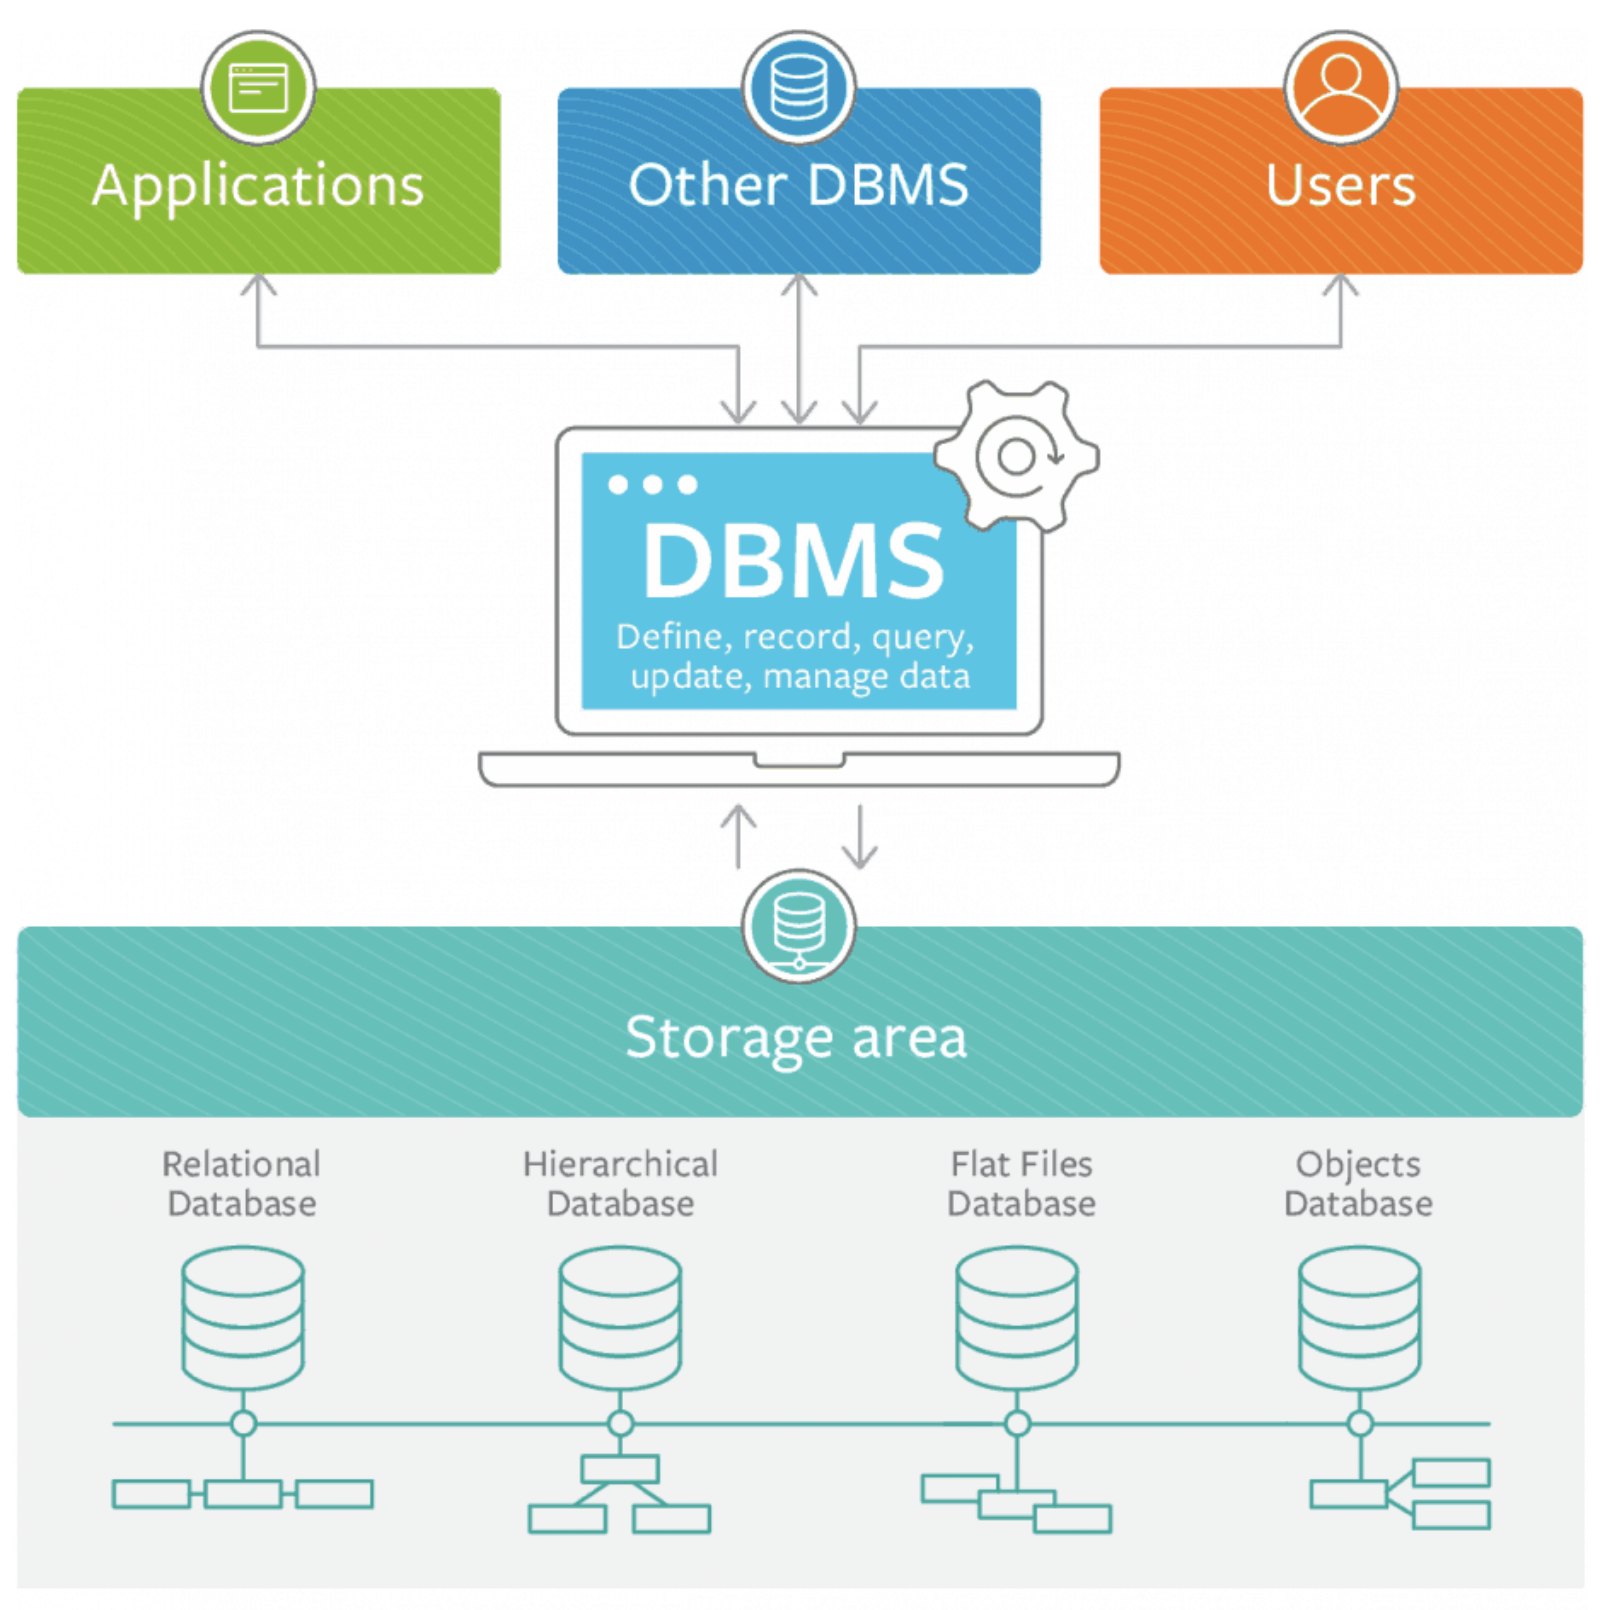
\includegraphics[width=0.5\linewidth]{figures/relational.png}
    \caption{Initial Database Management System Architecture.}
    \source{https://docs.chaossearch.io}
    \label{relational-db}
\end{figure}
They excel at maintaining data integrity through \ac{ACID} compliance but struggle with complex analytical queries across massive datasets. As \ac{BI} became critical, organizations transitioned to \textit{Data Warehouses}. These systems separate \ac{OLAP} tasks from operational ones to avoid performance degradation. While powerful, warehouses remain expensive and rigid, as they require data to be cleaned and transformed via \ac{ETL} before it can be stored. 
\begin{figure}[H]
    \centering
    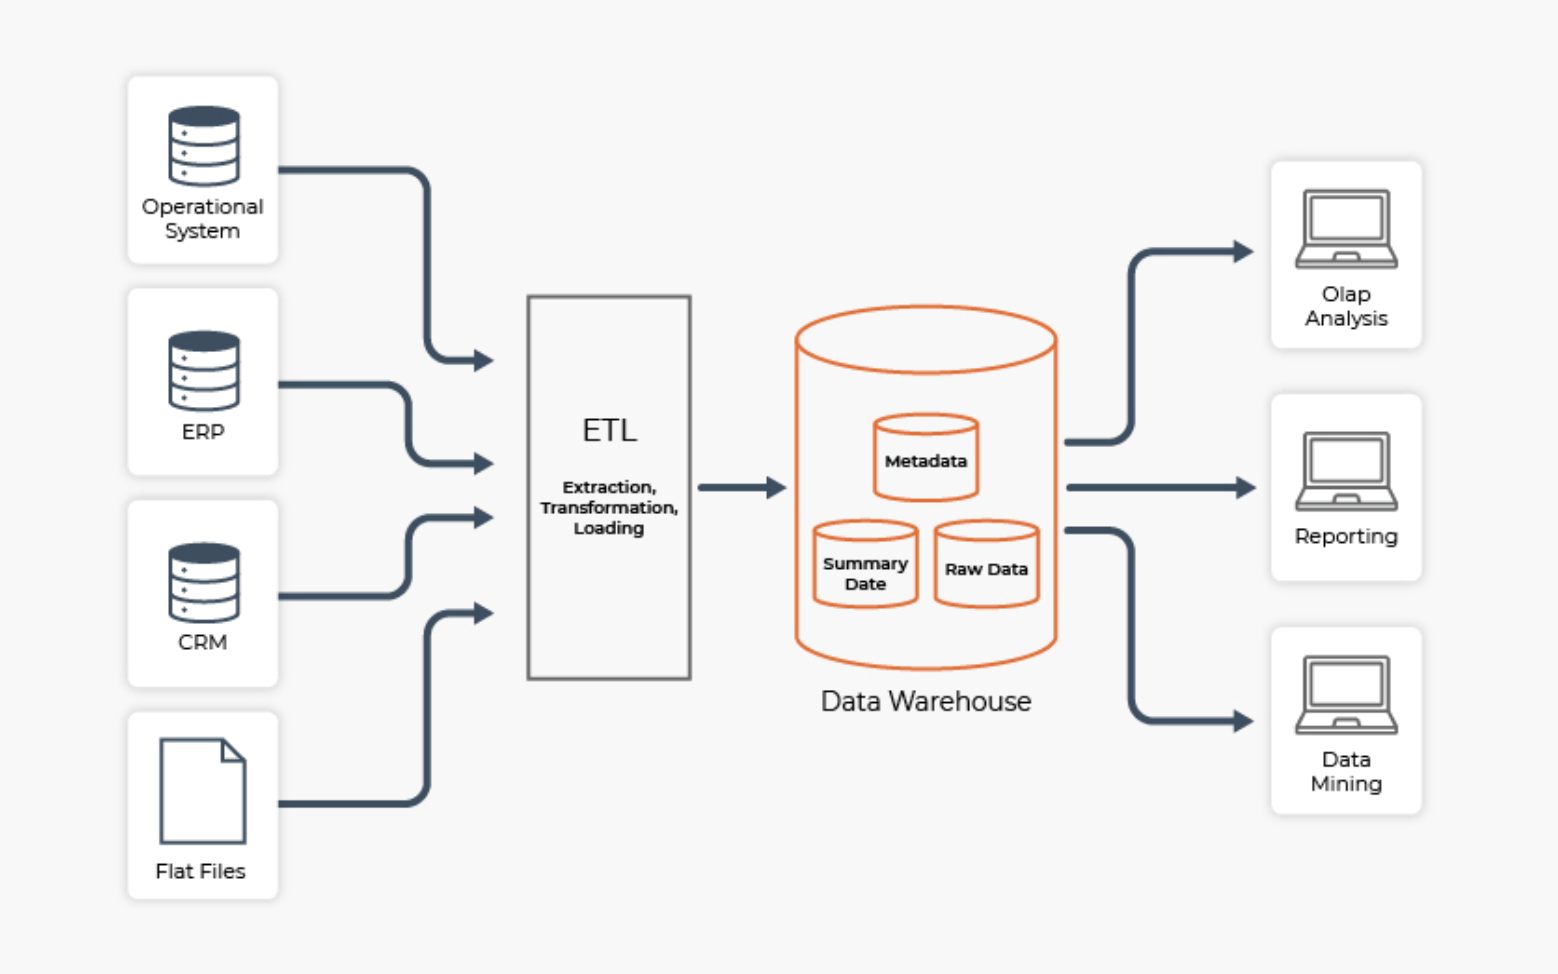
\includegraphics[width=0.5\linewidth]{figures/warehouse.png}
    \caption{Data Warehouse Architecture.}
    \source{https://docs.chaossearch.io}
    \label{warehouse}
\end{figure}

The explosion of \textit{Big Data} - characterized by high volume, velocity, and variety - led to the adoption of the \textit{Data Lake}. Unlike the warehouse, a lake serves as a central repository for raw data. This reflects a Schema-on-Read, because data is ingested without a predefined schema, avoiding the latency of upfront processing. Anyway, the risk is producing a \textit{Data Swamp}, because it can make data dirty due to the lack of structure even though it is highly flexible and cost-effective for storing massive telemetry logs. Consequently, the most recent architectural wave, formalized around 2021, is the \textit{Data Lakehouse}. This paradigm seeks to eliminate the inefficient ``two-tier'' architecture where data is duplicated between a lake (for Data Science) and a warehouse (for BI).
\begin{figure}[H]
    \centering
    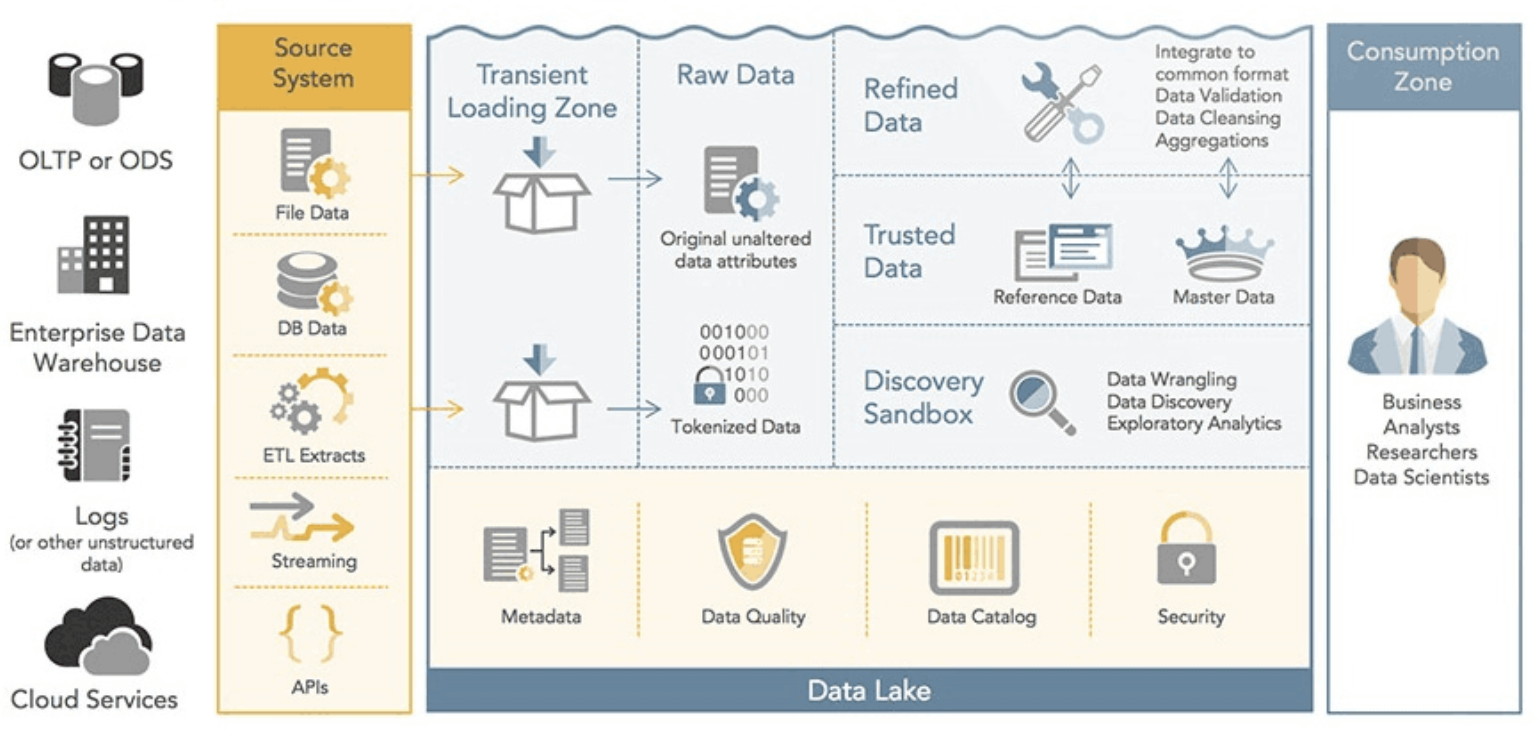
\includegraphics[width=0.5\linewidth]{figures/lake.png}
    \caption{DataLake Architecture.}
    \source{https://docs.chaossearch.io}
    \label{lake}
\end{figure}

The evolution from relational databases to Lakehouses was not merely a change in data structures; it was a fundamental shift in infrastructure philosophy. Traditional on-premise databases were vertically scaled, meaning that to handle more data, one had to buy a bigger, more expensive server. In the context of Technogym’s global expansion, this model became a bottleneck. The transition to cloud platforms (e.g., AWS, Azure, Google Cloud) provided the necessary substrate for modern observability to function. The secret of why cloud platforms work for observability is the decoupling of storage and compute. In traditional DBs, if we wanted to store 10 years of logs (storage), we also had to pay for the CPU (compute) to keep that server running 24/7. In the cloud we can store petabytes of \textit{cold} telemetry data in cheap object storage and only spin up powerful CPUs when we actually need to run a query or investigate a system failure.

The move to the cloud was driven by three main factors that differentiate it from the old ``Server in a room'' model:
\begin{itemize}
    \item Horizontal scalability: unlike a physical database, cloud platforms can distribute a single query across hundreds of virtual machines. This is vital for searching through billions of Mywellness app traces in seconds.
    \item Managed services (\ac{PaaS}): instead of Technogym engineers spending weeks configuring database backups and security patches, the cloud provider offers these as a service. This allows the team to focus on analyzing the telemetry rather than maintaining the pipe through which it flows.
    \item Global distribution: since fitness equipment is used worldwide, cloud platforms allow us to ingest data at edge locations close to the user, reducing latency and ensuring that observability does not slow down the user experience.
\end{itemize}

Ultimately, the cloud transformed the database into an Ecosystem. We no longer talk about a single tool, but an interconnected platform where eventually OpenTelemetry can send data to a collector, which routes it to a cloud-based Lakehouse, where it is finally visualized by an APM tool. The cloud is the ``glue'' that allows these modular components to communicate in real-time. Following the wave, Technogym already relies on AWS for storing the enterprise's data, in addition to Datadog used by the backend teams mainly for its storage capabilities, but actually contains loads of other useful features that will also be analyzed for our case study. 

Platforms like Datadog lead the attention to another characteristic that is worth mentioning before delving into platforms analysis: levels of outsourcing on the Cloud and, inherently, the principal vendors and possible architectures to adopt, that are the questions inspiring the research in the next chapter. 
Since the cloud is not a silver bullet, the decision to adopt it is not binary. The \textit{\ac{XaaS}} framework was born to allow organizations to choose their level of responsibility, effectively deciding which layers of the technology stack to manage internally and which to outsource to a vendor like AWS or Datadog. It goes without saying that this specific part will be useful for the considerations that inspire the platform research. It is helpful to distinguish some famous acronyms: 
\begin{itemize}
    \item \textbf{On-premise:} the traditional model where we would own the physical servers, networking, and storage in a local data center. It's best for highly regulated industries with extreme data sovereignty requirements or legacy systems that cannot be moved. The company would be in total control over the entire stack and data security. 
    \item \textbf{\ac{IaaS}:} the vendor provides the virtualized hardware (servers, storage, networking), but we manage the Operating System, middle-ware, and applications. It works for organizations that need high customization of the \ac{OS} or want to ``lift and shift'' existing apps to the cloud without redesigning them, eliminating hardware costs and scaling instantly. We are still responsible for security patches, \ac{OS} updates and runtime management.
    \item \textbf{\ac{PaaS}:} the vendor manages the hardware and the software framework (OS, middle-ware, runtime). We only manage the code and the data. It aligns with developers who want to build and deploy apps quickly due to high development velocity and lower operational overhead. Thus, because of the more predominant vendor lock-in, it can be tougher to move the code to a different provider if we use specific PaaS features.
    \item \textbf{\ac{FaaS}:} also known as serverless, a subset of PaaS where we deploy individual snippets of code (functions) that trigger on specific events (e.g., an OTel collector receiving a specific trace). It is the right choice for microservices or intermittent tasks that don't need a server running 24/7 and gifts extreme cost-efficiency since we pay only at code execution, but it also brings limited execution time and there is a bit of latency when the function wakes up. 
    \item \textbf{\ac{SaaS}:} the vendor provides a complete, ready-to-use application. We manage nothing but the configuration and the data we feed into it. It is addressed to specialized business needs like observability, CRM, or email where building a custom tool adds no competitive advantage. The advantages are zero maintenance, immediate access to advanced features, but it is the most expensive model at scale, it leaves the least amount of control over how the software works and pushes vendor lock-in to the extreme. 
\end{itemize}

 Another important concept to underline is called \textit{self-hosting}, that can be intertwined with on-prem. The latter refers to the physical location of the hardware, while the former puts the accent on the act of managing software ourselves instead of using SaaS. The twist is that we can self-host in the cloud by renting a blank \ac{VM} on AWS (\ac{IaaS}) and manually installing a database or an OTel collector on it without being clearly on-premise, because the server is the Amazon datacenter. These subtle questions have been discussed as they represent the holy grail to become familiar with the next steps. 

\section{The right platform: decision process} 

We can put the observability backend and the UX tool together in different ways. The realistic architectural solutions are:
\begin{itemize}
    \item \textbf{One-fit-all}: includes RUM, session replay, alerts, backend observability, and also supports OTel/OTLP export reasonably well.
    \item \textbf{Best-of-breed}: OTel-native backend for errors/performance/trace metrics and a dedicated UX/session analytics tool, stitched together via shared tags as \textit{session.id, user.id, page.url, etc}. 
\end{itemize}

\subsection{One-fit-all}

It means entrust everything to a unique platform, which would ensure workflow simplicity and linearity and less burden for components implementation. As already hinted, the best framed platforms were Datadog, New Relic and Sentry, which are about to be analyzed to understand the reasoning behind the process. 

From the official websites and related documentation, we can learn the analogies among the three that make them interchangeable \cite{Datadog,NewRelic,Sentry}:
\begin{itemize}
    \item The possibility of exploiting \textbf{session replay} functionalities with masking to respect privacy requests;
    \item The access to an EU data center (in Germany, Frankfurt), which reinforces the observance of specific legislation (\ac{GDPR}, AI Act, public DPA and consent and cookies policies for each);
    \item The usability of an integrated AI, even if some relevant differences will be fathomed in the following;
    \item Recognition of JS errors, React Error Boundaries, \ac{CWV} for RUM analytics useful for marketing strategies; 
    \item API call response time analysis for the frontend;
    \item Threshold definition and notification to automatically monitor anomalies, \ac{SLI}, \ac{SLO}, but it is a built-in functionality only in Datadog and New Relic, while Sentry needs support from other platforms;
    \item Geolocalization behind consent and GDPR best practices;
    \item Chance to add SDKs dedicated to full RUM, and these vendors offer their backend storage, which causes a higher vendor lock-in risk and less data portability (the limit is softened in Sentry's case thanks to the telemetry wrapper which introduces abstraction levels);
    \item They are not self-hosted, but \ac{SaaS}, further reason of vendor lock-in (Sentry could optionally be adopted as self-host, but this is not the conventional choice, and it is tougher to apply);
    \item All are OTel-supportive, but Sentry to a lesser extent; 
    \item Data retention period can vary on behalf of the plan and can be customized, but the default is a range of thirty days;
    \item Access control implementation, mainly for replays, generally adopting \ac{RBAC} or allow-list in Sentry.
\end{itemize}

However, we can also list the main differences among the three with a focus on Datadog, since it is the most complete. As a matter of fact, it is full-stack, that means we can save and correlate all signals emitted via native libraries in Datadog or via OTel SDK with OTLP in a single place. The classic data ingestion path can directly exploit Datadog's Agents or use an integrated cloud. Concerning the RUM path, we should use other SDKs to get complete analyses that the exclusive usage of OTel would not be capable of delivering. New Relic is the most complete platform after Datadog, but it is weaker about UX analysis with heatmaps and Datadog is slightly better in providing OTel-compatibility. Here, we can exploit the New Relic AI in addition to an \ac{SRE} Agent, but mostly to assist the user in error analysis and suggest remedies; therefore, it does not seem as powerful as Datadog's combination of Watchdog, for built-in insights, passive and automatic type of research, and bits AI SRE, which is added to the plan with additional fees but can conduct autonomous investigations, which is the extra value we wish to have. In Sentry, instead, the greatest lack is that OTLP insertion supports only traces and logs, not metrics and infra, so we should add a backend platform, which makes everything less doable. Furthermore, it does not directly build heatmaps and is less powerful for marketing metrics, only approximated through spans and replays. In fact, it is an excellent platform on the code and debugging side, which is a central but not exclusive part of our work. Another limitation in these terms is Seer AI, which is development-focused as debugging agent, which means it is not the best solution for our case. 
The cost model in Datadog is per host and follows ingestion and retention volumes, adding add-ons if any. The only critique against Datadog could be the risk of finding inflated costs at the end of the month. The model could be more transparent, so it requires more attention. New Relic and Sentry are safer, as they respectively follow an ingest-based and user model the former and an events-based and replay volume the latter. 

Datadog could be used following a Datadog-first approach to reduce external work, accelerating time-to-value, getting all the possible features, and correlations between frontend and backend. However, it requires more implementation effort to choose the RUM product (it could be Datadog itself using the SDKs or other specialized platforms like LogRocket or PostHog, which would be safer to have heatmaps and scrollmaps, too), manual correlation among tools through identifiers, alerting logic for the AI to intervene, and the storage in case we do not want to strongly depend on Datadog. OTel is still recommended for vendor-neutrality. 

\subsection{Best-of-breed}

Other than what involves Datadog said above, a common stack is the Grafana stack: \textit{Grafana} is the UI layer with dashboards, exploration, alerts, but it does not record telemetry, so it needs a backend beneath. It must be coupled with specialized components in interception of signals, like \textit{Tempo} for traces/spans, \textit{Loki} for logs, \textit{Prometheus} or \textit{Mimir} for metrics. The \ac{OTLP} in this context is feasible if adopting the collector to receive telemetry from the app, but the backend storage is detached. Interoperability is excellent, and this structure brings cost and control advantages, but pipelines and tools multiply. The only significant advantage with Grafana is making portable elements like dashboards and maps. The best-of-breed has never been fully considered because we did not want to complicate the system this much. Technogym already relies on SaaS, so the team was not worried about keeping this methodology. A percentage of vendor lock-in is welcomed if it keeps organization simpler. It was convenient because Technogym was already a Datadog's client \cite{Grafana}. 

\subsection{ClickHouse and the product ClickStack}

ClickHouse itself is a high-performance, column-oriented SQL database management system (DBMS) designed for online analytical processing (OLAP). It is available as both open-source and cloud-based offerings, optimized for running analytical queries over massive datasets in real-time. \cite{ClickStack} ClickStack, on the other hand, is the ClickHouse observability stack, an open-source platform built in collaboration with HyperDX. It is composed of three blocks: OTel collector (ClickStack distro), ClickHouse storage and its query system (with possibility to use something else), and ClickStack UI offered by HyperDX. ClickStack as a product can be used in two different configurations: as self-host so that we can manage it all, and a managed ClickStack embracing the SaaS approach, because we should manage the collector or any instrument we decide to use to send OTLP, ClickHouse and HyperDX are hosted and operated in ClickHouse cloud, and it is thought to scale and diminish the burden \cite{ClickHouse}.
\begin{figure}[H]
    \centering
    \begin{subfigure}[t]{0.45\textwidth}
        \centering
        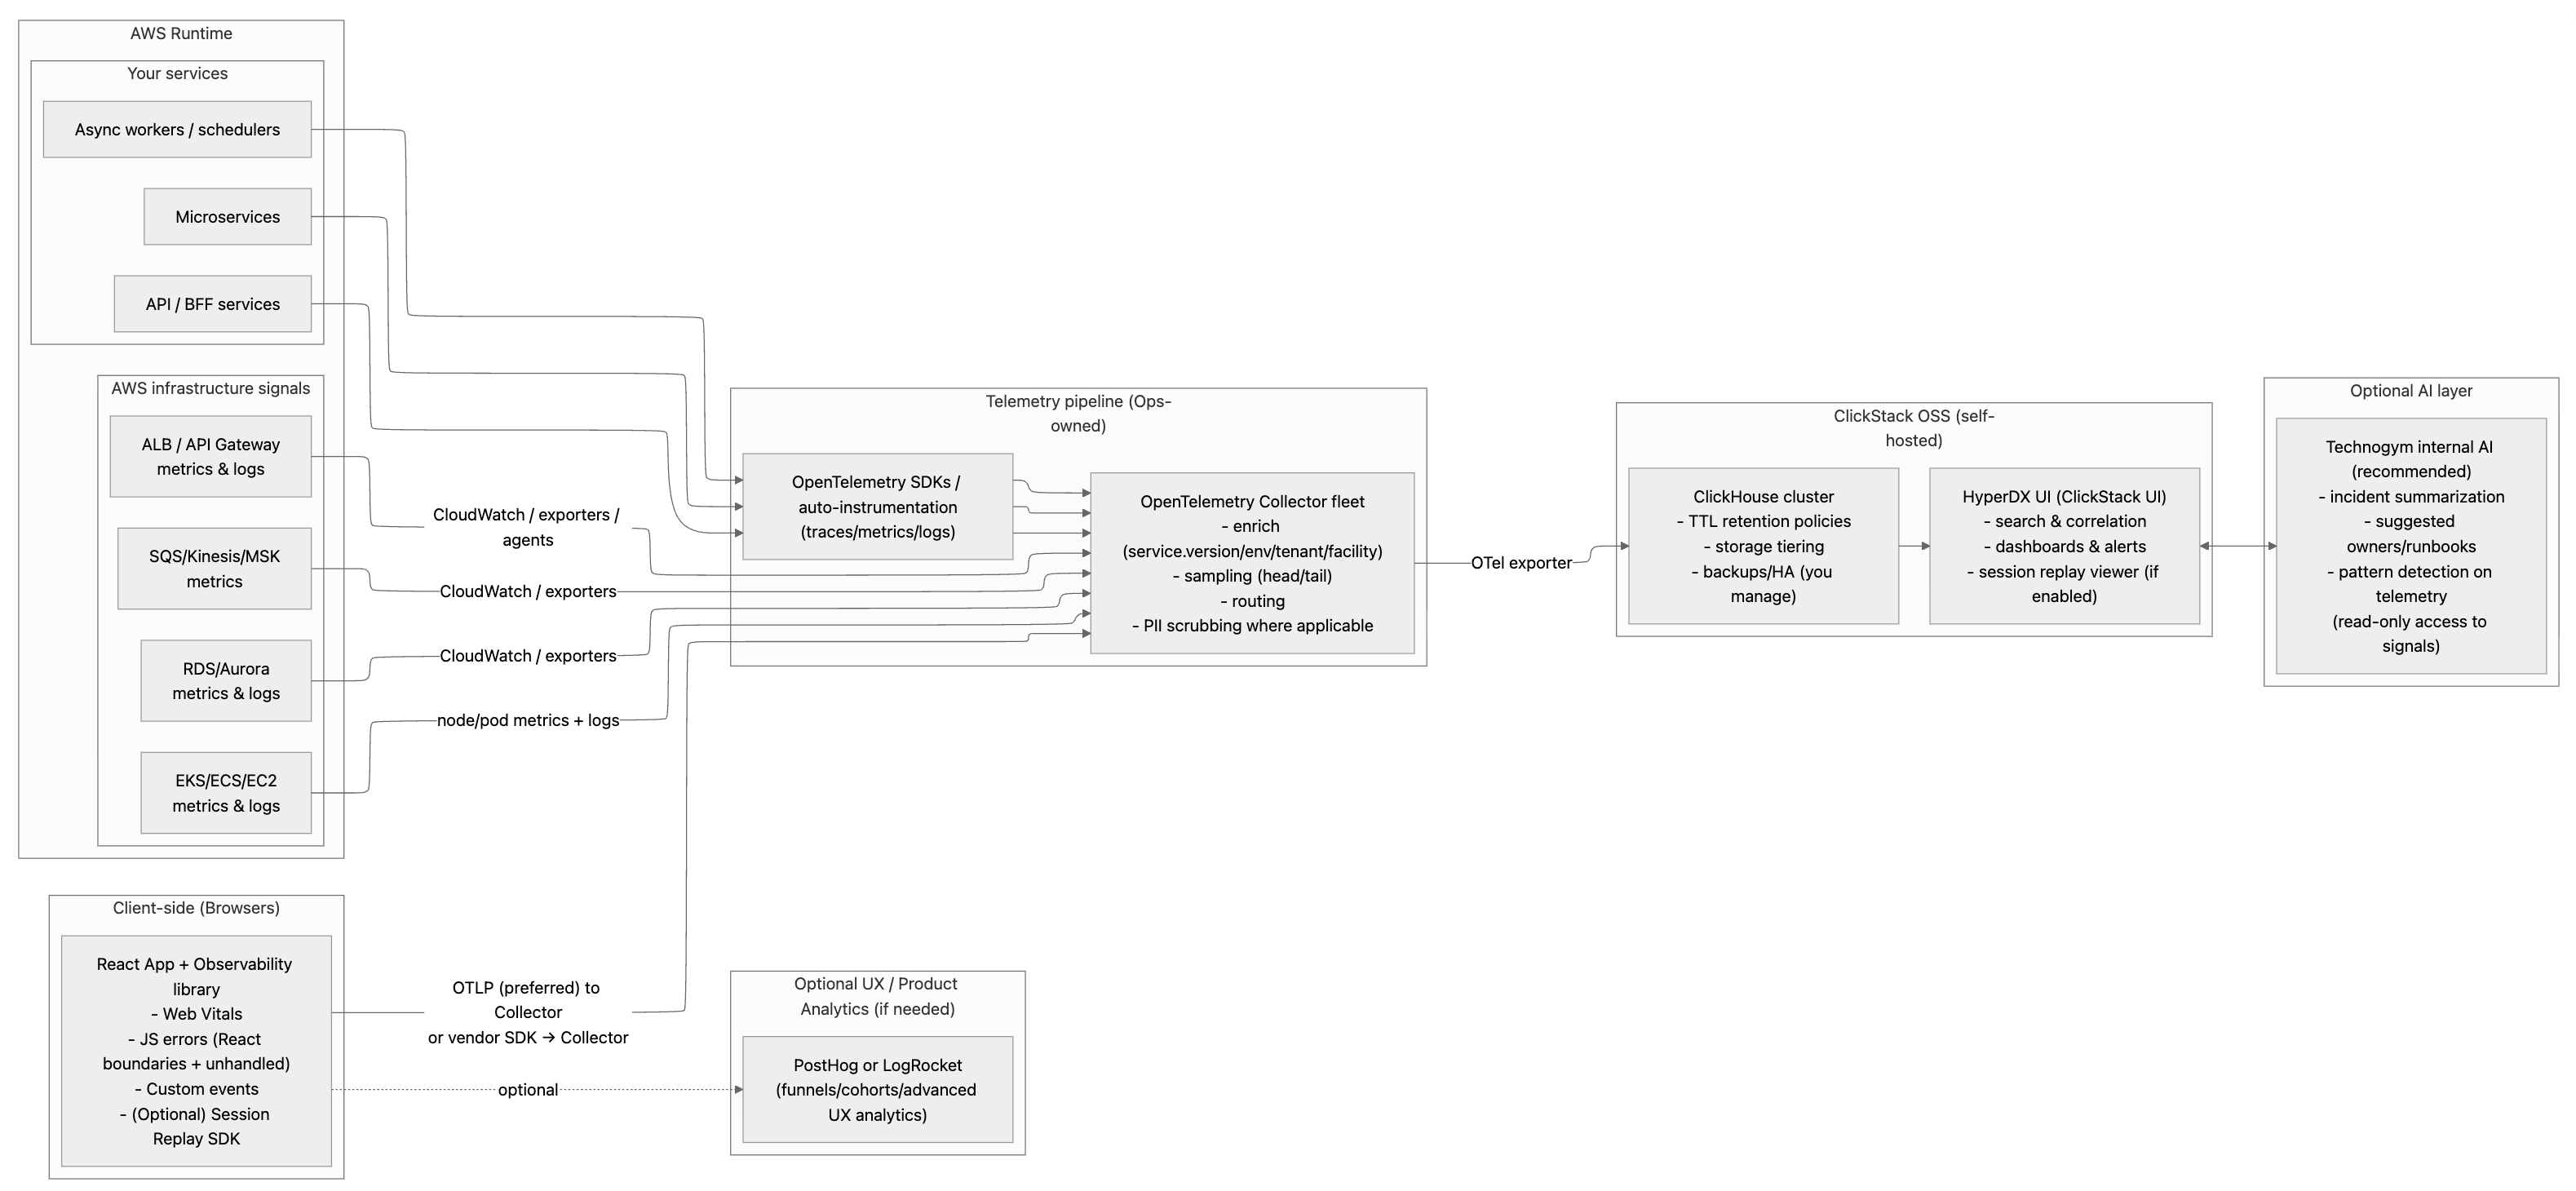
\includegraphics[width=\linewidth]{figures/osclick.png}
        \caption{Open-source ClickStack Architecture}
        \label{Open-source-Click}
    \end{subfigure}
    \hfill
    \begin{subfigure}[t]{0.45\textwidth}
        \centering
        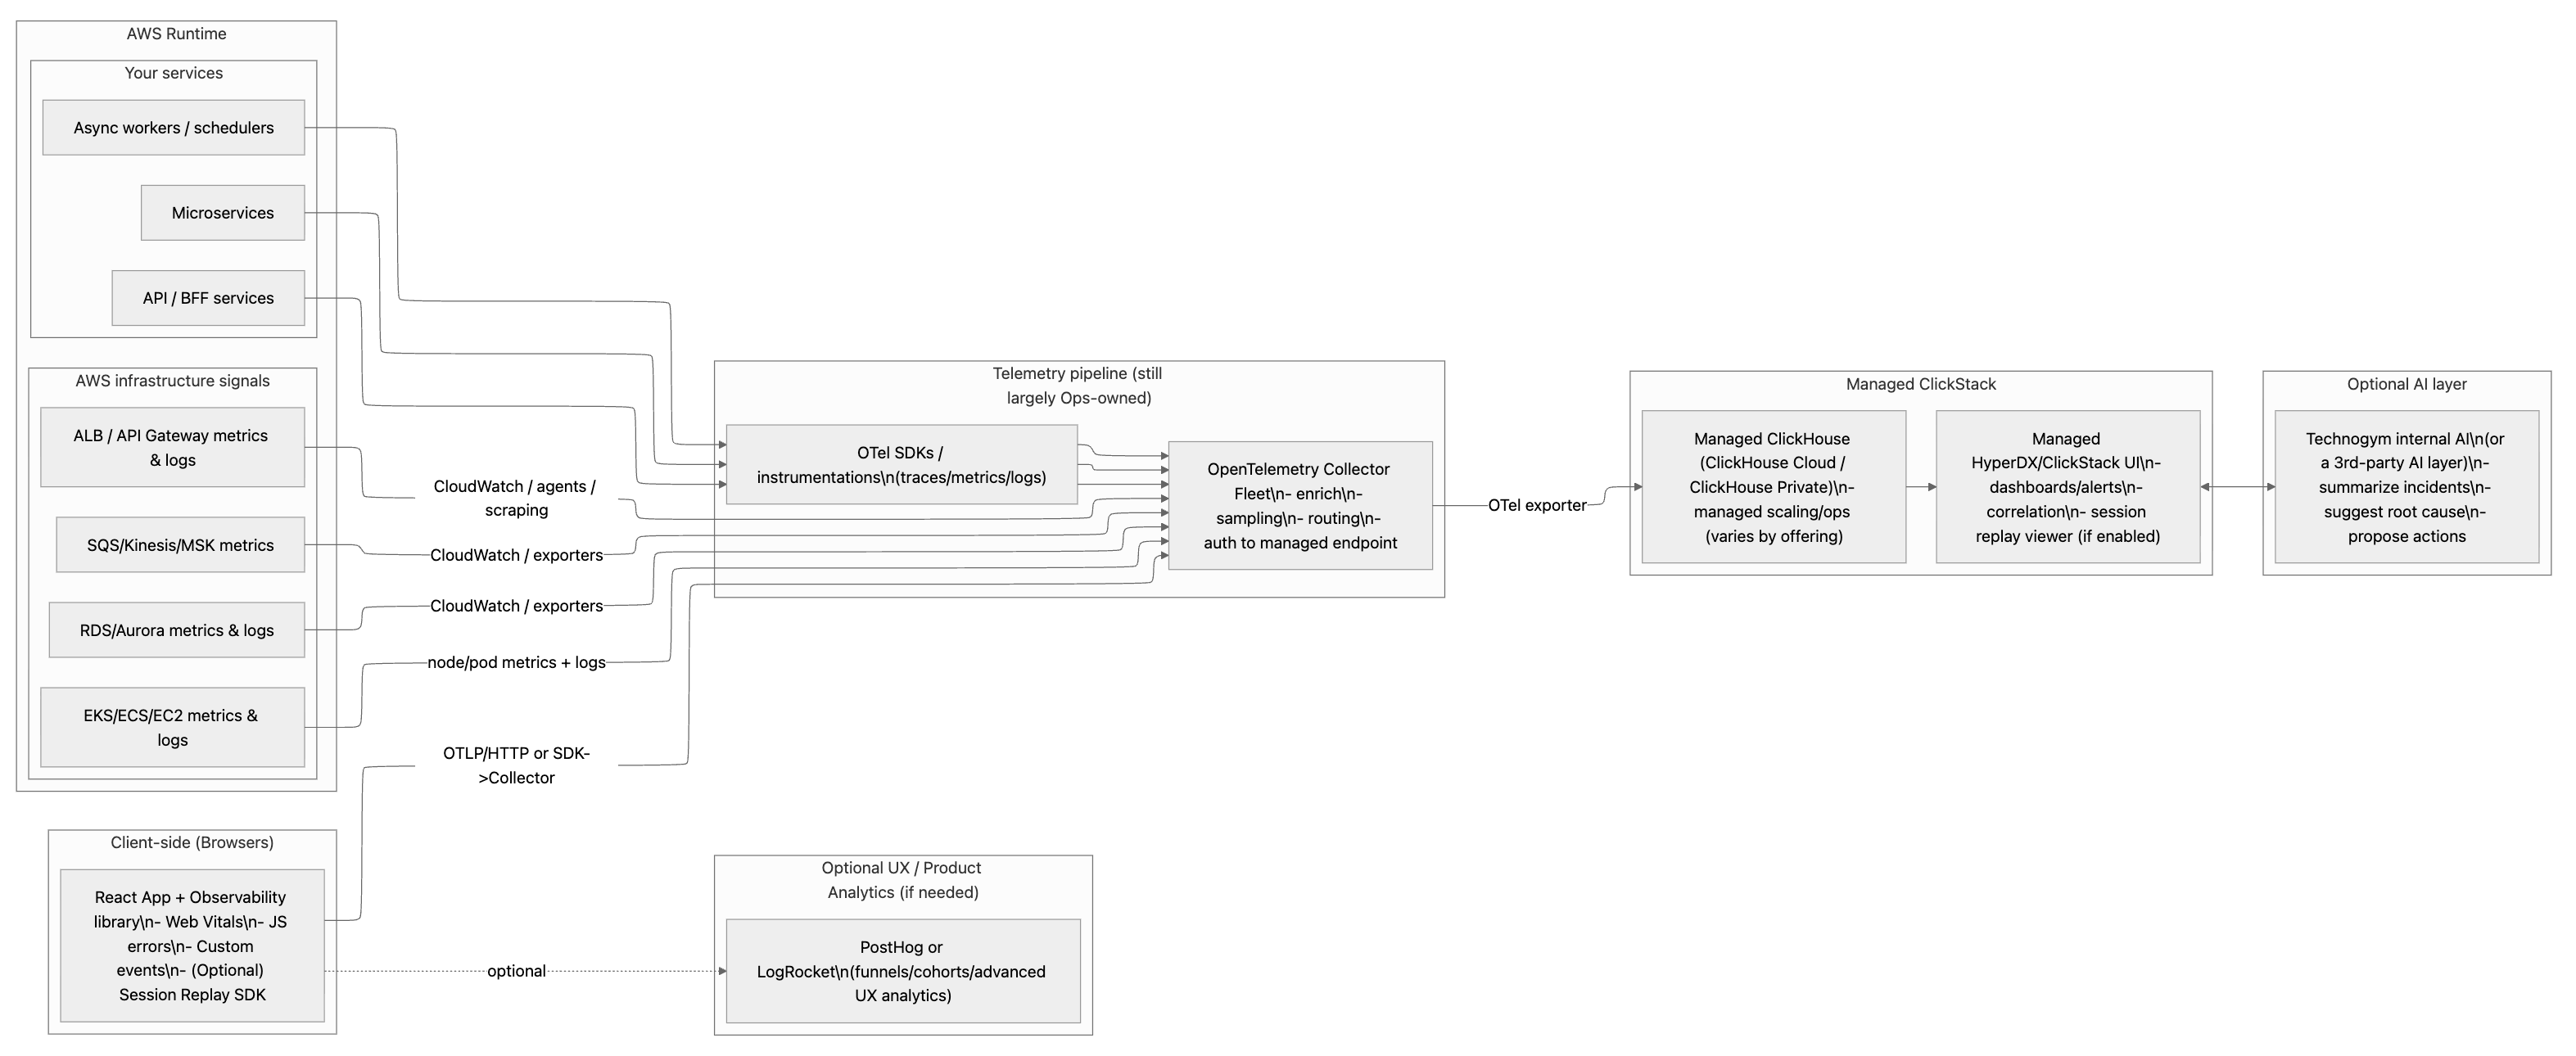
\includegraphics[width=\linewidth]{figures/Managedclick.png}
        \caption{Managed ClickStack Architecture}
        \label{managed-click}
    \end{subfigure}
    \caption{ClickStack Architecture Configurations}
\end{figure}
Technologically speaking, the two pipelines are significantly similar; operationally speaking, we skip the riskiest part in terms of \ac{MTTR}, because ClickHouse (or a general storage) is always on, we acquire the UI, authorization integrations and, most importantly, scaling. 

Even though the cost-model is incredibly tempting with ClickStack and ClickHouse (infra-based with promise of storage for less than \$0.03/GB/month and without fee per host), it brings some downsides with respect to Datadog. First of all, the AI is agentic, but only in the managed version and with the grant of a \textit{private preview} kind of account, hence owners decide who to leave the functionality to, and it is still work in progress, meaning we could experience changes in usage. The UI is not as developed as in Datadog, it offers many fair possibilities, but does not have heatmaps and it is base on static thresholds mainly, so to access dynamic alerts we should go for two integrated tools into HyperDX, that are \textit{Event Deltas} to analyze traces, and \textit{Event Patterns} to cluster similar log/traces. Plus, there is no explicit reference to \ac{CWV} capture. 

All these motives led us to confirming Datadog as the best solution, affirming again itself as probable leader on the market. 

\chapter{Practical implementation: from proof of concept to production integration}

In this chapter, we are going to dive into the practical implementation of the project. 

\section{Preliminary Test of ClickStack and Datadog}

The operational plan was generating the general telemetry setup to determine the structure and information we wanted any telemetry service to have, enabling the specific configuration for passing and managing telemetry through ClickStack and Datadog, and for completion improvising a demo page as interactive playground to test and verify telemetry collection from the simulated React application. Thanks to few simple buttons, it allowed to manually trigger various telemetry events and see them appear in real-time in the ClickStack UI.
The sections are:
\begin{itemize}[nosep]
    \item User context to set user identity for tracking user-specific telemetry (user id, email), but for privacy policy it should be masked or hashed, especially when checking session replays; otherwise, the risk is to go against the principles of the GDPR. In ClickStack's settings it is already possible to establish masking rules for sensitive data. It is important to link all telemetry events to a specific user for debugging user-specific issues; 
    \item Global attributes to add app-wide attributes that appear in all telemetry events (region, app version, browser) to reduce code duplication because it appears everywhere once set, enables filtering and grouping in the UI, and it is useful to correlate events across features;
    \item Logging (of types \textit{info} for general information message, \textit{warn} for something unexpected but recoverable, \textit{debug} for detailed debugging information usually disabled in production) and error tracking to record application events and messages at different security levels;
    \item Metrics to record quantitative measurements (counters, gauges, histograms) and simulation scenarios for realistic user workflows with multiple telemetry events at once (e.g., a user journey which simulates a complete e-commerce flow from searching the product to successful purchase); 
    \item User sign up at first account creation; 
\end{itemize}

As already hinted, we tested ClickStack to discover HyperDX's functions. We enabled the access to the local OSS version to avoid creating an account with a limited free trial time. With a ClickStack Docker VM instance, we could explore the interface freely, even though probably the experience in this way was not the same as the one we would have had via registration, and not all features were correctly accessible (such as the AI), but it was enough to grasp the general functioning idea. We formed our environment thanks to the ingestion API key to establish the direct connection with HyperDX, and configured the ClickStack local host endpoint. We used the standard ClickHouse ports to collect and pass telemetry. It already came with automatic browser instrumentation with fetch API calls tracked automatically, XML HTTP requests monitoring and user interactions. 

\begin{figure}[H]
    \centering
    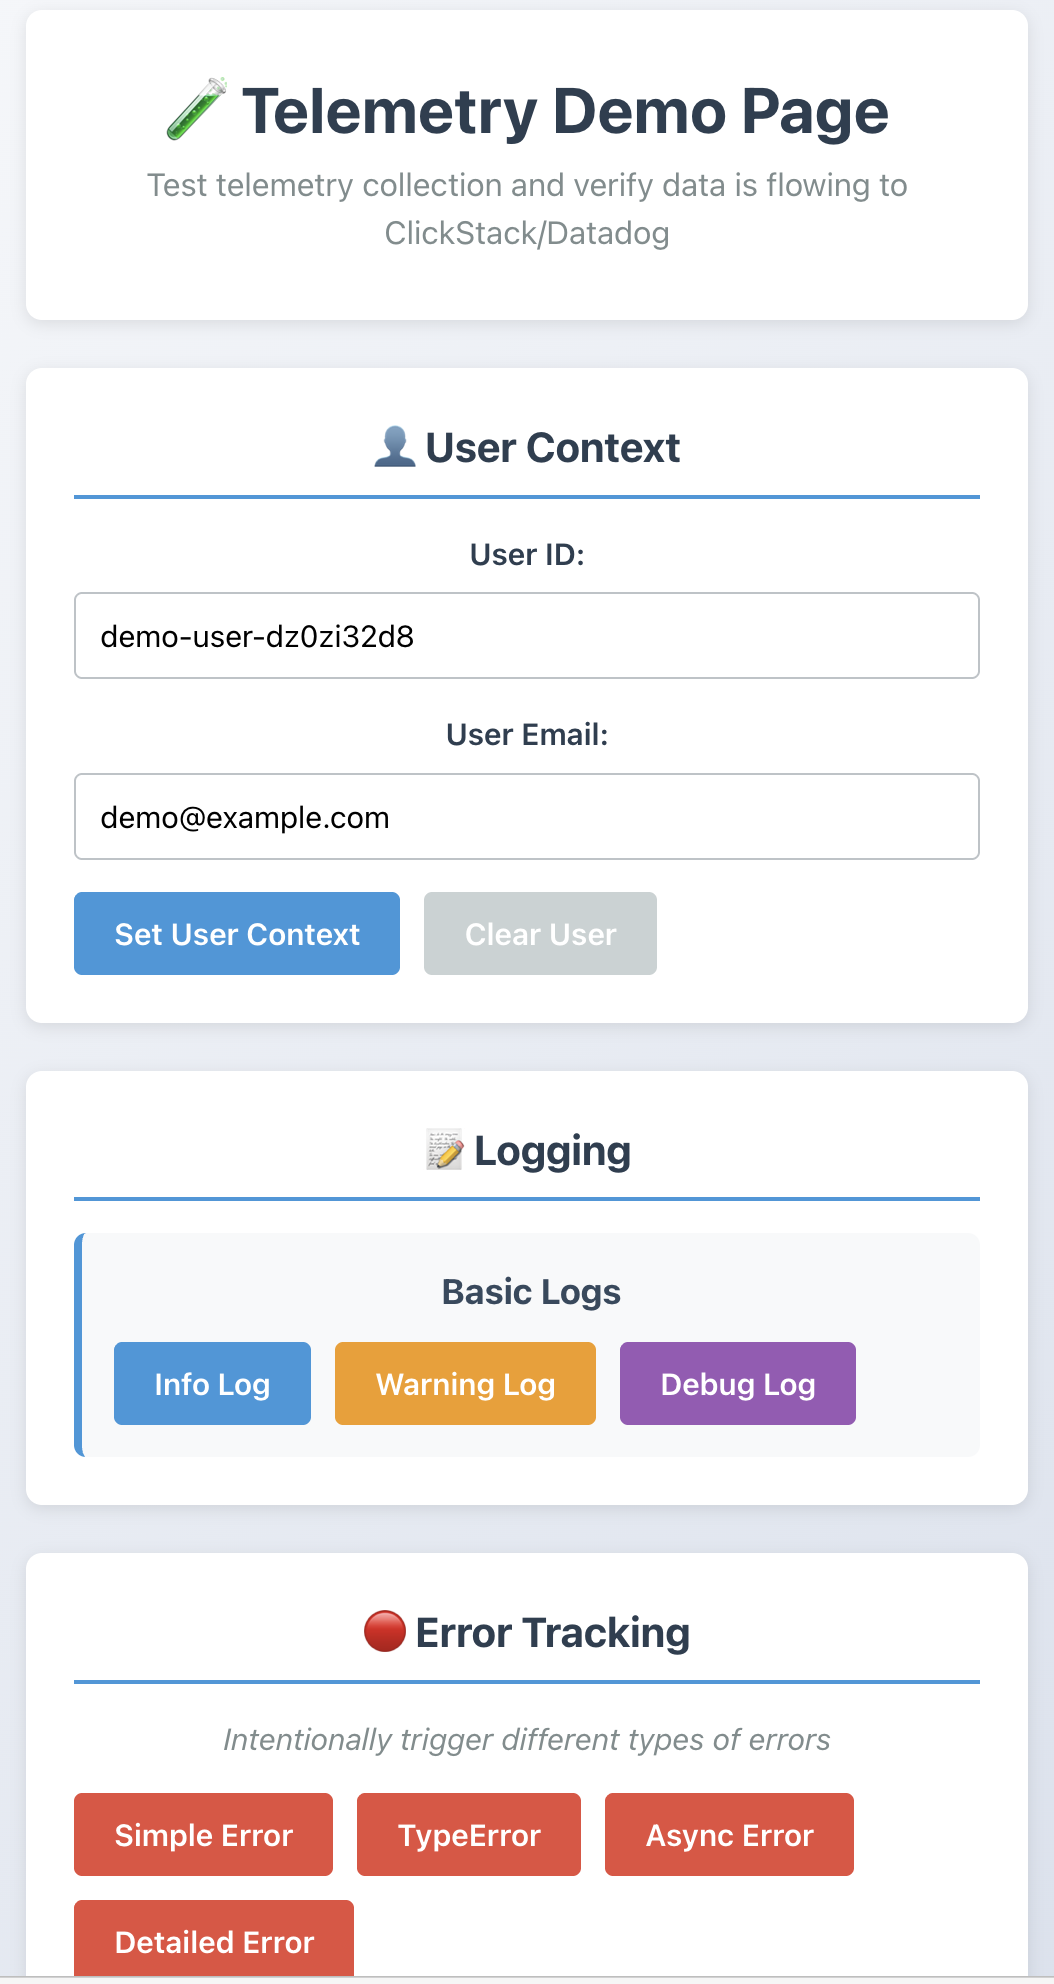
\includegraphics[width=0.3\linewidth]{figures/demo app.png}
    \caption{Demo App interface for reference}
    \label{demo}
\end{figure}

\begin{figure}[H]
    \centering
    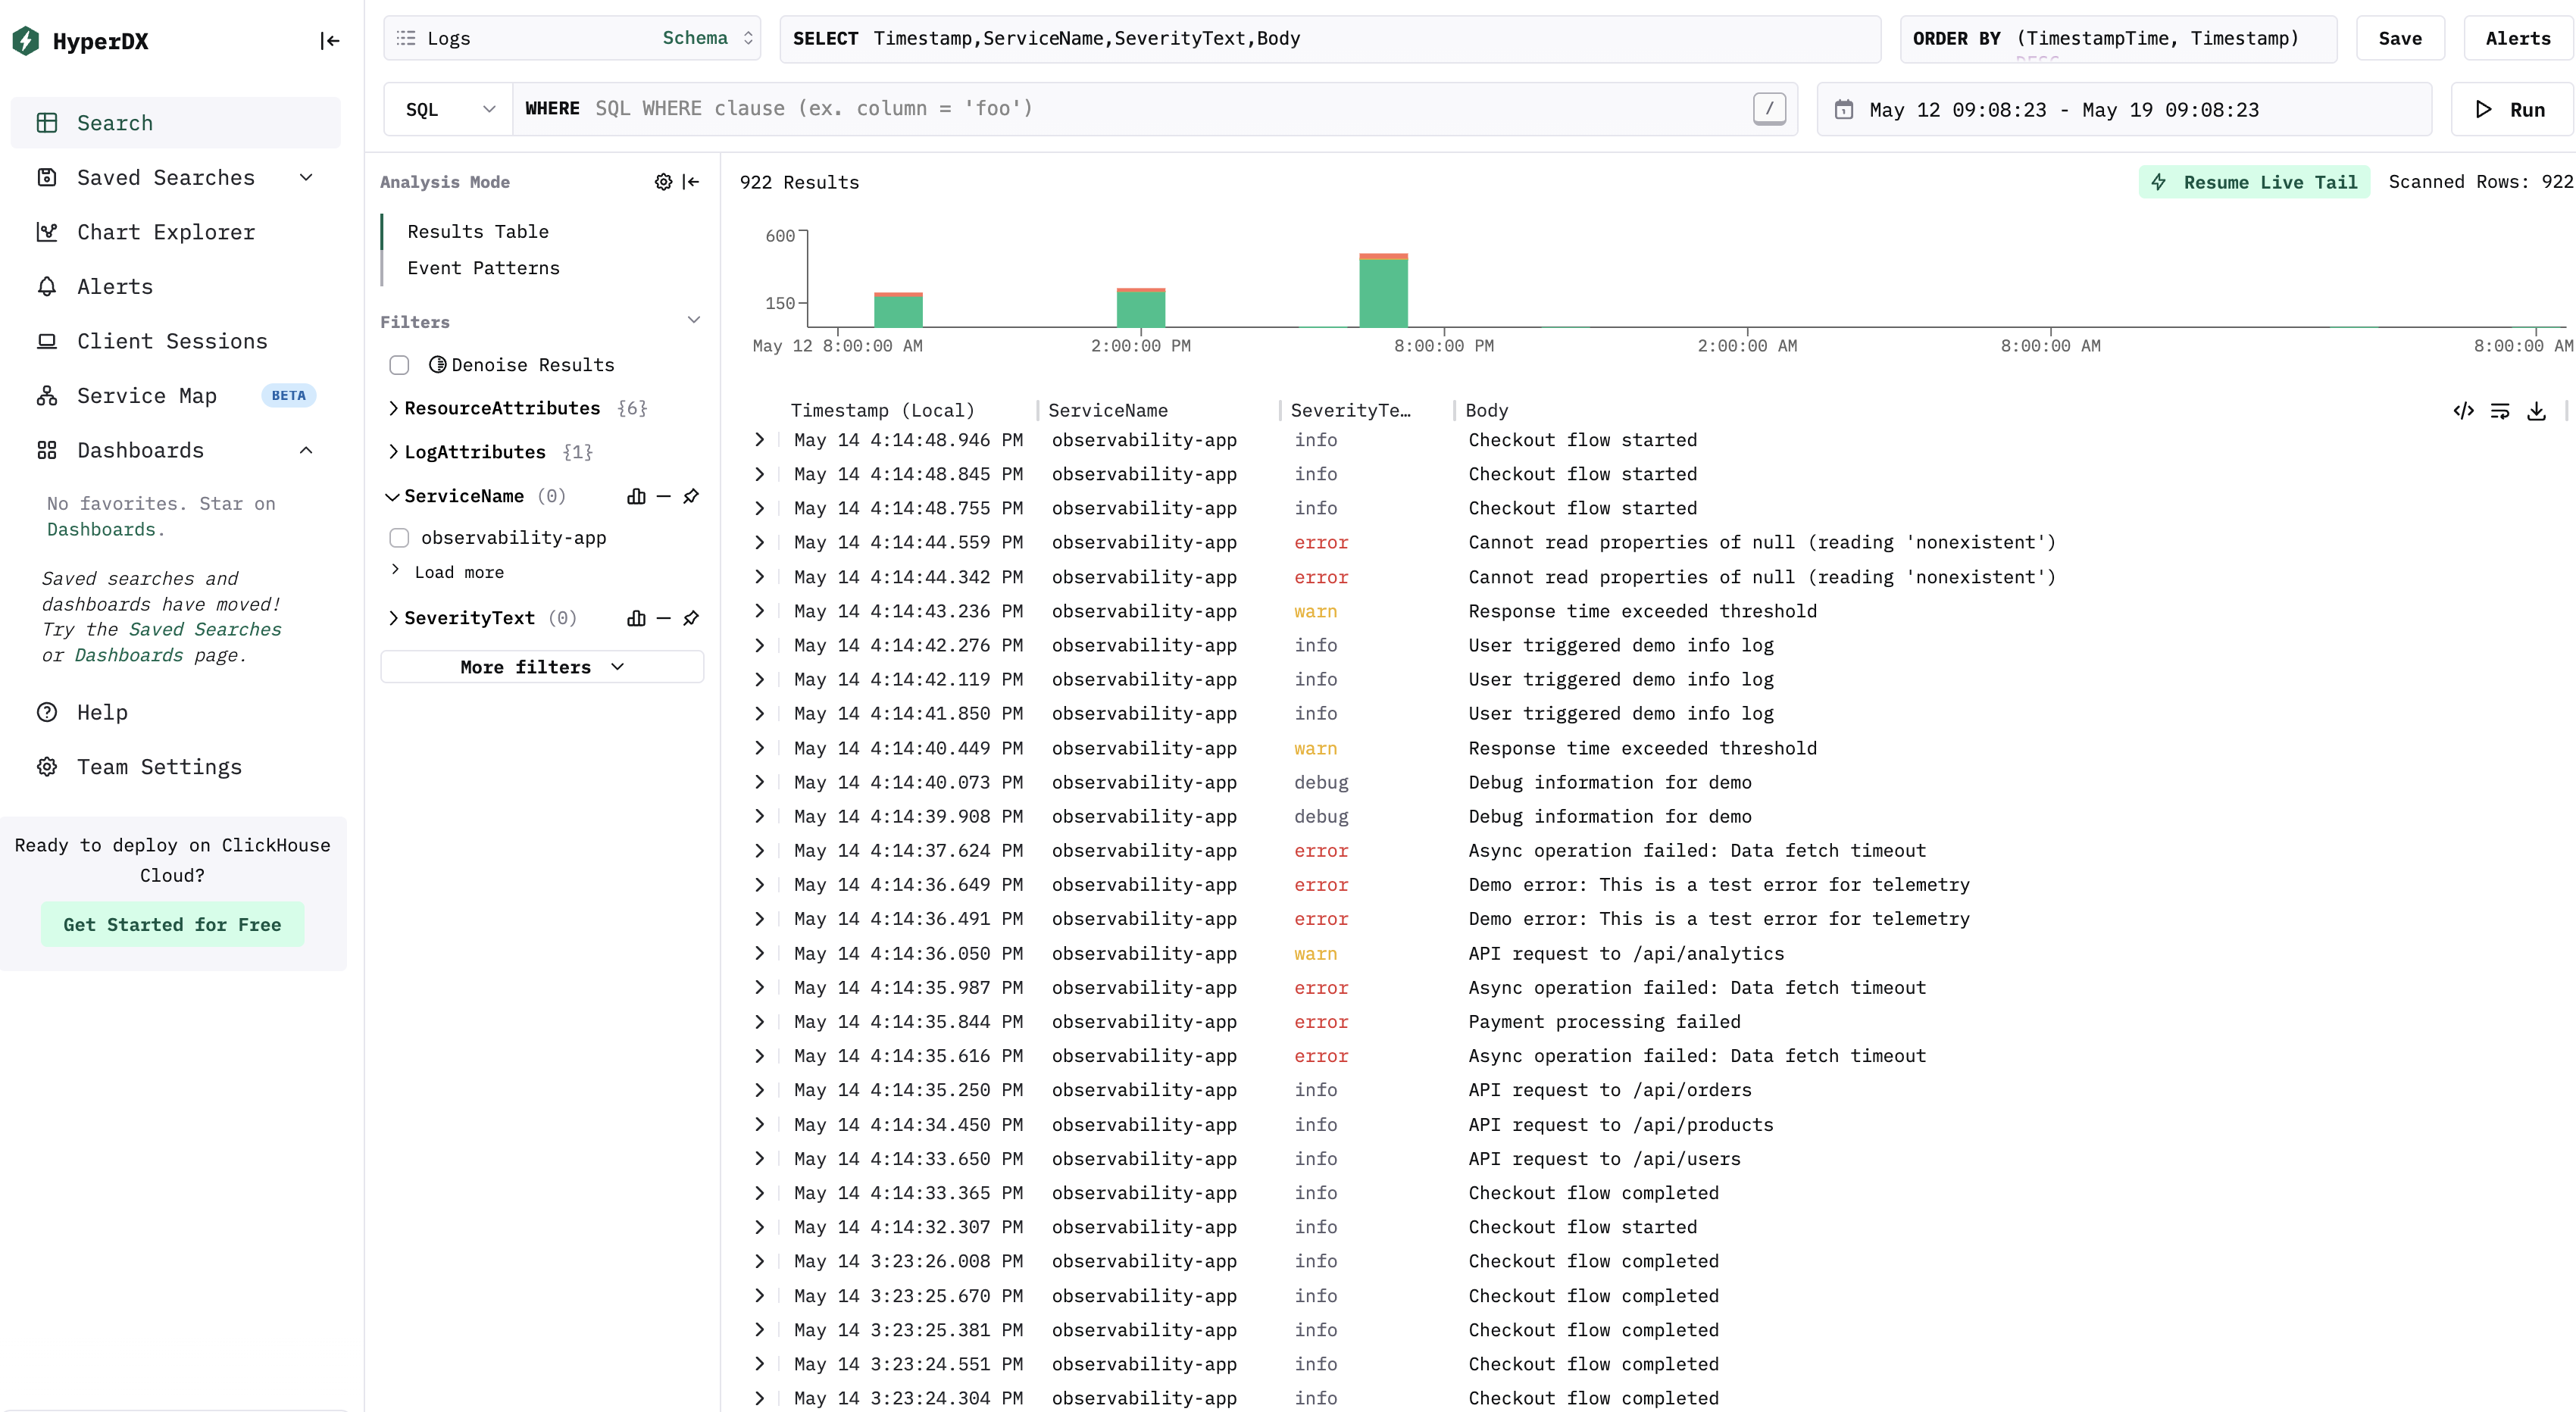
\includegraphics[width=0.8\linewidth]{figures/HyperDX interface.png}
    \caption{HyperDX interface: home page}
    \label{hyperdx}
\end{figure}

As we can see in this image (\cref{hyperdx}), thanks to the demo application, we have tested the collection of logs and traces in HyperDX, so that we could see the exact movements of the cursor of the user on the screen. By clicking on a specific row, we can visualize more detailed information in the form of tags that we used to write the SQL queries to build the dashboards. Some examples are:
\begin{figure}[htbp]
    \centering
    \begin{subfigure}[b]{0.55\textwidth}
        \centering
        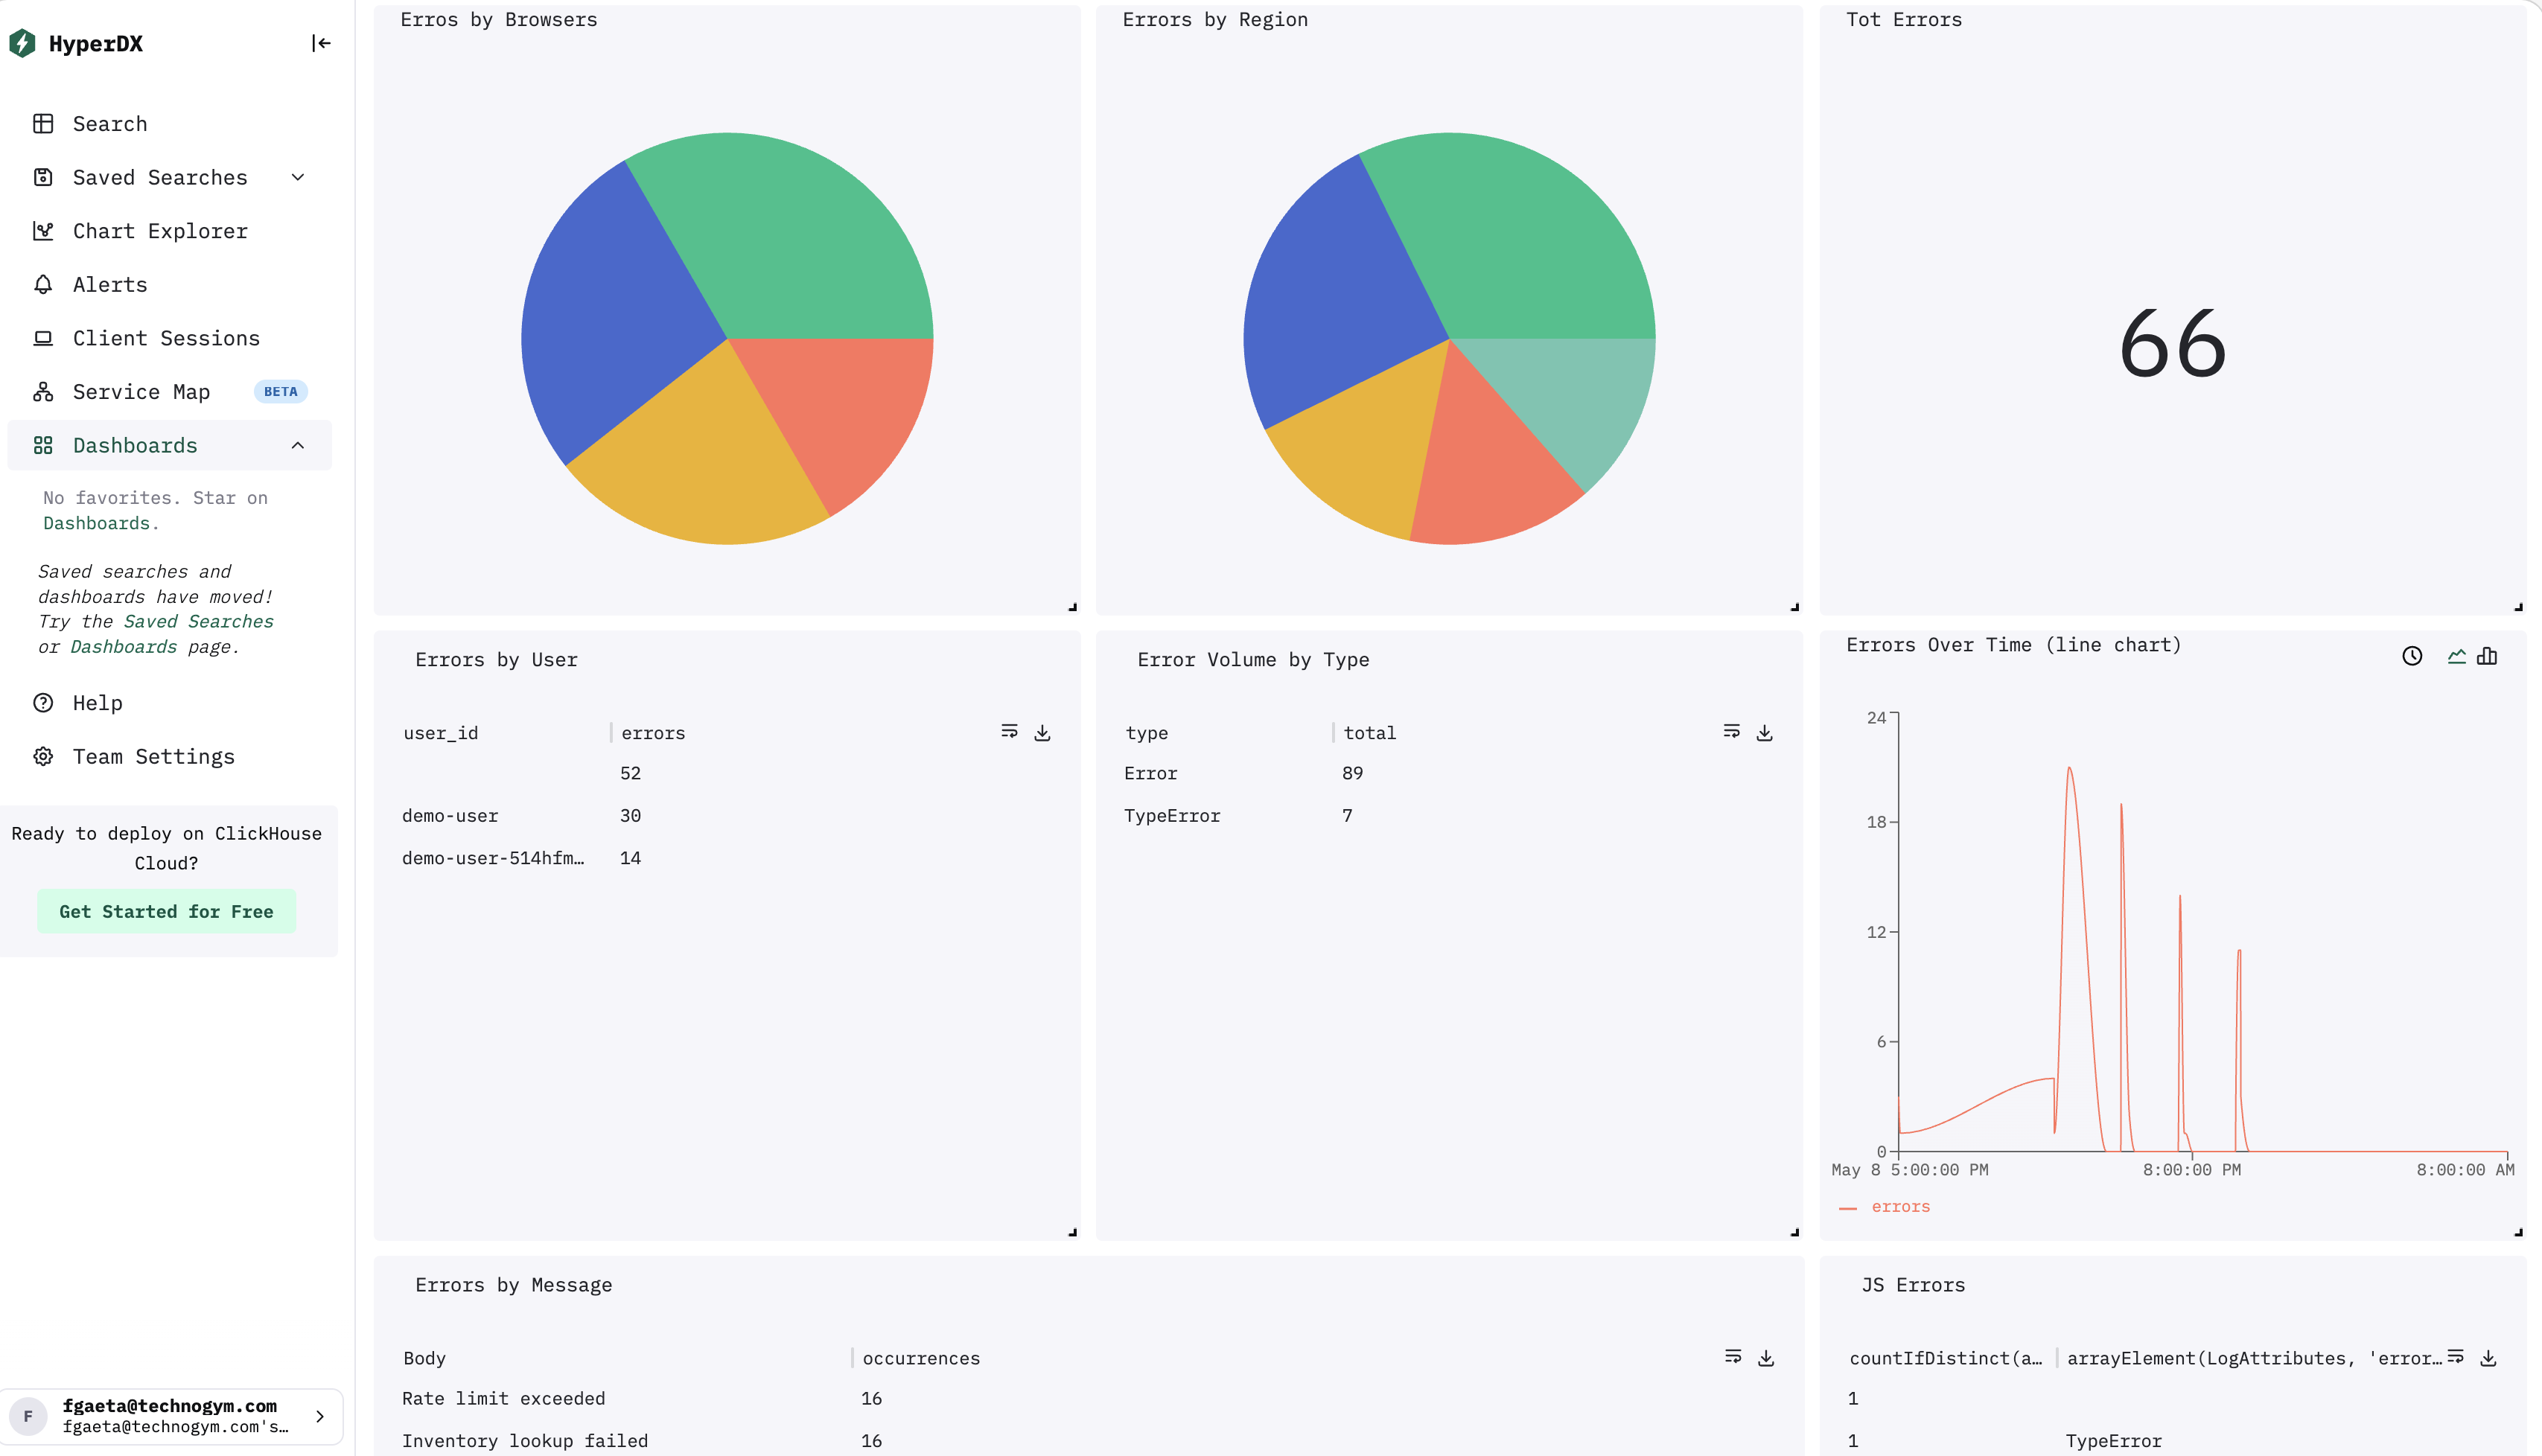
\includegraphics[width=\textwidth]{figures/dash HyperDX.png}
        \caption{Dashboards in HyperDX to Track Errors}
        \label{dashboard}
    \end{subfigure}
    \hfill 
    \begin{subfigure}[b]{0.37\textwidth}
        \centering
        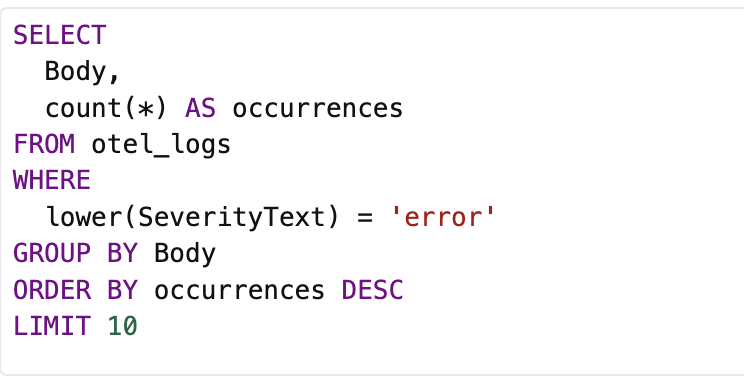
\includegraphics[width=\textwidth]{figures/SQL HyperDX.png} 
        \caption{SQL for Errors by Message}
        \label{sql}
    \end{subfigure}
\end{figure}

\section{Development standards for observability \\ integration in the source code}

The focal points concern the implementation of a new \textit{user story} dedicated to observability and the evolution of the modular architecture based on private packages. 

User stories represent specific units of work that need to be completed, such as developing a new feature, implementing tracking infrastructure, or fixing a bug. They are used to plan and schedule what modifications will be included in upcoming product released and can be tracked thanks to a platform called Jira. The team has established strict conventions to link these user stories directly to their Git workflow: 
\begin{itemize}
    \item \textbf{Branch Naming Convention.} When a developer creates a new branch for a single user story, the branch name must begin with the Jira user story ID, followed by an underscore and a brief description of the task. In our case, the specific ID was ``PROS-9099'' (written as: \textit{PROS-9099\_Observability}). 
    \item \textbf{Commit Message Convention.} The Jira issue ID must also be included inside the commit messages, typically placed in the footer section under ``refs''. By putting the ID in both the branch name and the commit message, the team can easily trace all code modifications back to the specific Jira issue they were intended to solve. This is particularly useful because when a task is too large, it is typically broken down into multiple user stories, instead of putting hundreds of IDs in the branch name, the team creates a single general branch, and by keeping the ID in the refs, we ensure the reference to the exact user story while underlining that all together aim to pursue the same objective. 
\end{itemize}

The development model is rigorously structured around a standardized branching model to guarantee the stability of production environments and flexibility for releases. The basic rule establishes that each new feature or correction should start from the branch \textit{main} (production source code). This strategy allows isolating changes and bringing them to production singularly. This is done to avoid the inclusion of non-tested functionalities in the release branch. 
\begin{table}[H]
\centering
\begin{tabular}{|p{0.2\textwidth}|p{0.4\textwidth}|p{0.3\textwidth}|}
\hline
\textbf{Branch Type} & \textbf{Description} & \textbf{Naming Convention} \\ \hline
Main & Source code in production & main \\ \hline
Dev / Test & development and inspection environments & dev, test, alfa, beta \\ \hline
Feature & New functionalities (with Jira ID) & feature/\newline JiraID\_BriefDescription \\ \hline
Release & Preparation for a new release & release/\textless name\textgreater \\ \hline
\end{tabular}
\caption{Git Branch Naming Conventions}
\label{branch_conventions}
\end{table}

Also, commits need to follow a semantic standard to facilitate traceability on Jira. The structure is \texttt{<type>(<scope>): <description>}, where types are drawn from the conventional commits list (feat, fix, docs, style, refactor...), the scope has been decided internally to indicate the part of the application that has been modified (home, planner, training...), in the footer we find the references field for the Jira issues.  

The application follows a modular philosophy, where components are interchangeable to reduce the dependency from specific libraries and to facilitate updates. The code is organized into reusable packages hosted in a private registry. The two main packages are ``Infrastructure'' with the basic logic, and ``Web App UI'' to manage UI components. The access to those requires authentication via private token locally configured in the NPM registry. 
The architecture is based on generic interfaces. For instance, the ``Tracking Service'' (initially referred to Google Analytics) is extended to the new Telemetry Service. The aim is not making the interface dependent on third-party libraries such as OTel, but these should be confined exclusively in the specific provider implementation (in our cases, ClickStack or Datadog). To achieve this, we defined a generic \textit{TelemetryService} interface. Instead of directly importing from OpenTelemetry API, we created custom generic types, such as a dictionary for attributes, where the key is a string and the value can be a string, number, or boolean, so the interface itself has zero dependency. This strict separation guarantees that if the team decides to stop using OpenTelemetry in the future, the core application interfaces will not need to be rewritten. The actual OTel logic is isolated within two specific implementation files, one regarding ClickStack for initial tests while waiting for Datadog's platform activation and exploratory sessions, and the other for using the latter. The necessary OTel packages are installed in the package.json as standard dependencies rather than development dependencies, ensuring that they are included in the final compile application build.  

\subsection{Page views tracking, sanitization and \\ session replay towards GDPR compliance}

Once the telemetry abstraction layer has been introduced, the next step consisted in instrumenting the application to collect navigation events. Sending metrics, logs and traces was quite trivial, since we just had to import the code we had prefabricated in the demo app and apply some refinements to integrate it with the existing components. Another observability feature implemented through the new architecture was page views tracking, again taking inspiration to the already done work. Page views are essential telemetry signals to jump into user navigation flows and to allow the construction of usage analytics dashboards. To reach this goal, the activity focused on automatically tracking route changes throughout the application. 

The tracking logic was centralized: instead of embedding telemetry calls inside individual pages which would cause \textit{scattering} (literally spreading things over a wide area, hence calls towards tracking systems would be lost in the whole business logic, making each modification onerous and error-prone), the implementation leveraged the telemetry service abstraction and centralized page view registration within the routing layer. This approach reduced code duplication and guaranteed consistent event generation across the entire application. The \textit{trackPageView} method uses the parameter ``path'' instead of the complete URL. This must be brought to attention because while the URL (composed of \textit{window.location.href}) might include protocols and hosts, the \textit{path} identifies the logical internal path (e.g. /people/contacts). This choice was made for privacy protection to avoid the unintentional capture of PII (Personal Identifiable Information) or sensible query parameters. What we did is called \textit{sanitization}.

\begin{lstlisting}[language=Kotlin, caption={sanitization function}, label=lst:sanitization]
    export function sanitizePath(path: string): string {
  return path
    .split('/')
    .map(segment => {
      // Check if segment is a GUID (with or without dashes)
      // Pattern: 8-4-4-4-12 hex digits or 32 hex digits without dashes
      const isGuid = /^[0-9a-f]{8}-?[0-9a-f]{4}-?[0-9a-f]{4}-?[0-9a-f]{4}-?[0-9a-f]{12}$/i.test(segment)

      // Check if segment is a MongoDB ObjectId
      // Pattern: 24 hexadecimal characters
      const isObjectId = /^[0-9a-f]{24}$/i.test(segment)

      // Check if segment is purely numeric (IDs like 123, 456)
      const isNumericId = /^\d+$/.test(segment)

      // Replace GUIDs, ObjectIds, and numeric IDs with :id
      if (isGuid || isObjectId || isNumericId) {
        return ':id'
      }

      return segment
    })
    .join('/')
\end{lstlisting}


Sanitization links to the concept of data cleanliness, too. Sending row data to monitoring systems is not only risky in privacy terms, but could additionally cause a technical issue known as ``cardinality explosion''. If dashboards receive tons of univocal entries, their statistical aggregation becomes unfeasible, making data unavailable for operational monitoring. The usage of a GUID (Globally Unique Identifier) composed of 32 characters by default separated by dashes in URL paths prevents metrics' grouping. It means that every access to a specific resource would be seen as a different page because the user has changed. Sanitization is the only way which allows operators to visualize traffic as aggregated per sections. For instance, /contacts/UUID-123 turns into more generic /contacts/ID. In the code we can find a sanitization function in the telemetry utilities which exploits regex to identify not only GUIDs, but also numerical and more compact ``object IDs'' typically returned by databases. These identifiers get replaced with a generic ``ID'' which guarantees cleanliness across sent data.

This procedure is a must to comply with the \ac{GDPR} and other privacy regulations that end up being very impactful especially in the European context. 
The GDPR governs the collection of personal data within the EU territory. Its objective is defining what sensitive data is, how it can be collected, how to deal with biometric data which is another subset of the wider sensitive information group, and how to protect the privacy of individuals. 
\cite{GDPR} In art.4, we encounter the definition of \textit{personal data} as any information relating to a natural person, also known as data subject, identified or identifiable, directly or indirectly, by reference to an identifier such as name, ID number, location data, or more factors specific to the physical, physiological, cultural (...) identity of that person. 
Enterprises must pay attention to the \textit{principle of data minimization}, which states that personal data must be adequate, relevant and limited to what is necessary in relation to the purposes for which they are processed. In our case, it means we should not send any PII to the telemetry system, and we should avoid sending any sensitive data that could be used to identify a user. 

Since we wanted to track user navigation flows and revise them in session replays, it was mandatory to implement a masking strategy to hide sensitive information, which leaded us to obscuring the input fields for usernames and passwords, address, telephone number, birthdate and so on. Consequently, we also needed to reach the same results for dropdown menus used to select sensitive information, such as the birthdate through the common date picker interface. In the original code before bringing my edits, Mouseflow was the tool used for user interactions granular monitoring. The system utilized the \texttt{SensitiveInfoClassName} constant (defined as \texttt{sensitive\_info}) and the boolean \texttt{sensitive} prop to mark components that need to be hidden. Among these elements, profile pictures are also included, considering that platforms are generally not able to autonomously understand which images need to be covered as sensitive content. Mouseflow also prevented data capture at the source, masking information directly on the client-side to avoid any risky transmission, considering that post-processing would be actually forbidden according to the company's Zero-Trust Data Egress policy. 
Datadog RUM, instead, offers advanced instruments for privacy management, but the configuration must be calibrated in order to reflect the severity of our current system. Datadog provides two approaches for marking sensitive content: HTML attributes (data-dd-privacy=``value'') or CSS classes (dd-privacy-value). The available privacy levels are:
\begin{itemize}
    \item \textbf{hidden:} the content of the element is not captured in the session replay, and it is replaced with a placeholder such as a gray rectangle, which is the safest solution since it does not even let third parties know the number of characters and words in the field;
    \item \textbf{mask:} the content of the element is captured, but it is masked with dots or asterisks, which means the length of the content is visible, except for the actual characters, rendering the wireframe. It is the best compromise between privacy and usability, but we could privilege ``hidden'' because there is nothing to be gained from knowing the length of a password or a username for our debugging purposes;
    \item \textbf{mask-user-input:} the content is captured, but the user input is masked with dots/asterisks while the rest of the content is visible, so that we can only obscure what is sensitive. 
    \item \textbf{allow:} the content is simply captured and displayed in the session replay.
\end{itemize}

Our final strategy was adopting the CSS class approach, maintaining the existing \texttt{sensitive\_info} class to ensure backward compatibility. This allowed all tags already marked with the \texttt{SensitiveInfoClassName} to automatically benefit from Datadog's privacy masking without requiring modifications to hundreds of component instances. Subsequently, by navigating different parts of the app and reviewing the session replays, we continued adding the class where needed but where there was no previous reference to the sensitive information props. 
The default privacy behavior in Datadog initialization was set to 'allow', because it would have been significantly more complex to explicitly allow the hundreds of non-sensitive elements, compared to selectively masking the dozens of sensitive components, the majority of which were already identified. 

\subsection{Performance monitoring: legacy and new APIs \\ and Core Web Vitals}

\cite{perfmon} Performance monitoring concerns the systemic process of tracking, measuring, and analyzing key performance indicators to ensure goals are being met, and evaluate the progress and effectiveness of an application in this specific case. The guidelines for the project were to keep \acp{CWV}, page and resource loading time and React component rendering performance under control, besides analyzing API call response time. 

\cite{API} \acp{API} are the invisible backbone of modern software development. They enable applications and systems to communicate and share data efficiently with seamless interactions among platforms, services and applications. The API takes a request, sends it to the server, retrieves the data and then returns the response. 

\begin{figure}[H]
    \centering
    \includegraphics[width=0.5\linewidth]{figures/api.png}
    \caption{API Request-Response Cycle.}
    \source{https://www.geeksforgeeks.org/software-testing/what-is-an-api}
    \label{api-cycle}
\end{figure}

There are numerous types of APIs we could mention, but in our case study what is relevant is studying the \textit{RESTful APIs}, which are based on the principles of Representational State Transfer (REST). RESTful APIs use standard HTTP methods (GET to retrieve a record, POST to create a new one, PUT to update it, PATCH as a partial update, DELETE to remove the record) to perform operations on resources identified by URLs. They are stateless, meaning each request from a client to a server must contain all the information needed to understand and process the request. RESTful APIs are widely used due to their simplicity, scalability, and compatibility with web technologies. In our context, it is essential to understand the error categories that can be returned by the server in response to a request. These are represented by three-digit HTTP status codes that start from 4xx to 5xx. For instance, some of the most common mistakes that can be experienced by normal users are error 404 (Not Found), error 403 (Forbidden), error 401 (Unauthorized) and error 500 (Internal Server Error) or 503 (Service Unavailable). The 5xx category is the most dangerous because it indicates a server-side problem that prevents the request from being fulfilled, while the others concern client-side criticalities. Furthermore, we can encounter network errors (timeouts, connection refused), or custom business logic errors, which return a 200 status code (OK) even when the request is not successful, and the error payload attached should be investigated to verify if there is something wrong and where. 

The latter is particularly crucial in our architecture. The old legacy APIs are managed with an explicit comment at code-level to check if there is an "error" array despite the 200 OK response. This was a common practice to separate HTTP errors from applicative errors, to distinguish when a request fails from when it arrives correctly, but the operation failed for business reasons. The new APIs, instead, are designed to return a 4xx or 5xx status code when an error occurs, following the standard HTTP conventions. This change improves the clarity of error handling and allows for more efficient debugging and monitoring of API interactions; as a matter of fact, the following steps involve a transition to the new ones. The migration of API legacy is a tactic necessity dictated by the \ac{EoS} of current servers, estimated for the beginning of next year (2027). There are two possible ``versioning APIs'' strategies teams can choose between, but right now they are adopting V1 which is a more trivial redirect, because with respect to the V2 strategy it is faster thanks to the fact that there is no need to re-create the API from scratch, but the input and output will stay the same so that the test phase is faced quickly, the impact on the client is null since touchpoints are not affected and the transition is transparent. The result is a new infrastructure maintaining the legacy code, while in V2 a new paradigm with a new code would be introduced. The V2 strategy is still in the to-do list, but it is a long-term strategy that requires time, effort and risk for mistakes, therefore it is essential for now to minimize the impact on the client and accelerate parity tests.

\begin{lstlisting}[language=Kotlin, caption={API error handling}, label=lst:api-error-handling]
import HttpResponseMessage from './../../http/models/HttpResponseMessage';
import HttpStatusCodeType from './../../http/models/HttpStatusCodeType';
import RepositoryResponseError from './RepositoryResponseError';

declare class RepositoryResponse<TData> {
    data?: TData;
    errors?: RepositoryResponseError[];
    token?: string;
    tokenNotValid: boolean;
    permissionDenied: boolean;
    mfaRequired: boolean;
    statusCode?: HttpStatusCodeType;
    constructor(
        httpResponse?: HttpResponseMessage,
        responseIsInBody?: boolean,
        responseMapper?: (data: any) => TData
    );
    get hasErrors(): boolean;
    getErrorMessage(): string;
    private getGenericError;
}

export default RepositoryResponse;
\end{lstlisting}

The \ac{BE} teams - managing API calls, connections to databases, AI integration to work with data - were already exploiting Datadog in four main areas: \ac{APM} for all microservices, infrastructure and cloud monitoring to collect metrics from the underlying AWS infrastructure, alerting for critical reliability signals, logs and async processing with archive search for historical investigation. 
When \ac{BE} and \ac{FE} are monitored in isolation, the views for each are disconnected even if they concern the same user journey. The FE lives through RUM and the BE through APM, and this creates a gap. By reaching the goal of linking RUM sessions to backend traces, we get an end-to-end view. The correlation works through a distributed tracing context injection so that the RUM SDK ingests trace headers into every HTTP request to the backend. 

\begin{lstlisting}[language=Kotlin, caption={RUM SDK trace context}, label=lst:trace-cont]
datadogRum.init({
  applicationId: '<APPLICATION_ID>',
  clientToken: '<CLIENT_TOKEN>',
  site: 'datadoghq.com',
  service: 'professional-next',
  allowedTracingUrls: [
    "https://services.mywellness.com",
    /^https:\/\/[^\/]+\.mywellness\.com/
  ],
  trackResources: true,
  trackLongTasks: true,
  trackUserInteractions: true,
});
\end{lstlisting}

To show the chain, we need RUM configured with \textit{allowedTracingUrls} to know which calls to correlate, and W3C trace context propagation \textit{traceparent} to link the BE trace to its child. \ac{CORS} should already be configured to allow such headers, because the backend has to accept them due to security rules. \cite{CORS}Indeed, \ac{CORS} is a mechanism for integrating applications by defining a way for client web applications that are loaded in one domain to interact with resources in a different domain. This is useful because complex applications often reference third-party APIs and resources in their client-side code. 
This is needed because any kind of discomfort that the client might experience while using the CRM Mywellness application is perceived as an interface/application error, even when it is not a responsibility of frontend programmers, but the common user has no technical expertise to understand it, hence their feedbacks will sound generic, too. Without this proper traceability methdology, we would waste a lot of time looking for the source of the problem almost randomly checking code files. 

\cite{CWV} \acp{CWV} is a set of metrics that measure real-world user experience for loading performance, interactivity, and visual stability of the page. The categories we are interested in refer mainly to the user experience impact: 
\begin{itemize}
    \item \textbf{LCP (Largest Contentful Paint.)} It tracks how fast the main content loads, which can correlate to retention rate because, if the users abandon slow sites, retention is directly affected negatively. 
    \item \textbf{FID/INP (First Input Delay/Interaction to Next Paint.)} It is about responsiveness of the elements. At the beginning there was only FID, which measures only the time of the first user input to start the interaction, this is why nowadays is often sided or replaces by INP, which is about the total response time that comprehends all interactions, which can be more useful in application contexts. 
    \item \textbf{CLS (Cumulative Layout Shift).} It concerns visual stability. If there are unexpected layout shifts, it can lead to user errors or general poor \ac{UX}, which discourages people to use the app. 
\end{itemize}

To qualify as "good" performance, Google establishes the following thresholds: LCP should occur within 2.5 seconds, INP should be below 200 milliseconds, and CLS should remain under 0.1. These targets must be met for at least 75\% of page visits. For Technogym, establishing these benchmarks as \ac{SLI} allows the team to define clear \ac{SLO} and trigger alerts when performance degrades, enabling proactive intervention before users experience significant impact. Integrating CWV monitoring into the observability infrastructure provides real-time visibility into user experience across different devices, network conditions, and geographic regions. Through OpenTelemetry's browser instrumentation, these metrics can be correlated with backend traces, allowing the team to identify whether a poor LCP stems from slow API responses, excessive JavaScript execution, or network latency. This end-to-end visibility transforms CWV from isolated frontend metrics into actionable insights that guide both frontend and backend optimization efforts.

\section{Sarà la sezione su dashboard datadog etc.}

In this section, we will explore the creation of dashboards in Datadog. In order not to disclose private information, I am going to use images and references that head for the test environment and mocked local interactions, not real users sessions (which will be available in the final part of the full internship). 

Throughout the process, it has been decided that the priority for the enterprise was to intercept errors with severity labeled as ``critical'' and ``high'', because it is the biggest pain point for the company in terms of customer care and application quality.  



%----------------------------------------------------------------------------------------
% BIBLIOGRAPHY
%----------------------------------------------------------------------------------------

\backmatter

\bibliographystyle{unsrt}
\bibliography{bibliography}

\begin{acknowledgements} % this is optional
This thesis represents the end of one of the most beautiful, despite hard at times, journeys of my life, thanks to the new, fascinating things I have studied and the wonderful people I have met. 

First of all, I am grateful to my supervisor, Professor Matteo Francia, not because it is a formality, but because he has truly been a great mentor, capable of explaining complex concepts while also having fun with his students at the end of his lectures, because he is both a great professor and person, he has eased our study path with his humor and, specifically to me, he has been a psychological support, too, helping me every time I had doubts about my next steps. A big thanks also to my co-supervisor, Davide Domini, who since the first year has been mainly a friend, he helped me to solve all the endless bugs in my terminal and always knew how to encourage me. 

The most important thanks go again and always to my family. I know that, for you, I am the perfect daughter that can do whatever she can, but it is not true, and I have never felt this way towards myself. But I also know that if I am brave, ambitious and stubborn enough today to think I can face two years studying informatics to realize my childhood dream and survive six months of programming for an internship, it is because you raised me making me feel the love and safety I needed to be able to take risks, knowing I could have never disappointed you because you would have been always proud of me even committing the worst failure of my life, and because after all your sacrifices you deserved me to try hard, and I hope to give you my success as a gift every day.

The best feeling was finding colleagues that I have always called friends. From those who came into my life during the Bachelor's and never left, Alessia, Tommaso, Cinzia and Greta, to all my DTM fellows and the new people I met. You were able to make me discover new traits of my personality, new activities to enjoy, new objectives to pursue, you were always ready to support me even when I was unsure about everything and just overthinking my next ten years of life. As I already told you, I could endure other thousands of university courses with you, because you are the best medicine for my mind and my soul. It destroys me to think I won't see you every day anymore and that we are all going to be scattered around the world, but I know you are the kind of people that find a way to see each other and keep on with our adventures as we left the day before. Thank you for the esteem you show me, it is completely reciprocated, and I know you will be extremely successful. You will always feel like home and I deeply love you. 

\end{acknowledgements}

\end{document}
